\documentclass[12pt,a4paper]{report}

% ─── حزم اللغة والخطوط والاتجاه ───
\usepackage{fontspec}
\usepackage{polyglossia}
\setmainlanguage[numerals=maghrib]{arabic}
\setotherlanguage{english}

% تعيين خط عربي قياسي متاح على كافة الأنظمة
\newfontfamily\arabicfont[Script=Arabic,Scale=1.1]{Arial}
\newfontfamily\arabicfontsf[Script=Arabic,Scale=1.1]{Arial}
\newfontfamily\arabicfonttt[Script=Arabic,Scale=1.0]{Courier New}

% ─── حزم الأبعاد والهندسة ───
\usepackage[a4paper,top=2.5cm,bottom=2.5cm,left=2cm,right=2cm]{geometry}
\usepackage{fancyhdr}
\usepackage{titlesec}
\usepackage{xcolor}
\usepackage{graphicx}
\usepackage{subcaption}
\usepackage{caption}
\usepackage{booktabs}
\usepackage{tabularx}
\usepackage{array}
\usepackage{amsmath,amssymb}
\usepackage[most]{tcolorbox}
\usepackage{hyperref}

% مسار مجلد الصور
\graphicspath{{figures/}}

% ─── ألوان الهوية البصرية الرسمية ───
\definecolor{StudioPrimary}{HTML}{0284C7}
\definecolor{StudioSecondary}{HTML}{4F46E5}
\definecolor{StudioDark}{HTML}{0F172A}
\definecolor{StudioLight}{HTML}{F8FAFC}
\definecolor{StudioBorder}{HTML}{E2E8F0}
\definecolor{StudioGreen}{HTML}{10B981}

% ─── إعدادات الروابط التشعبية ───
\hypersetup{
    colorlinks=true,
    linkcolor=StudioPrimary,
    citecolor=StudioSecondary,
    urlcolor=StudioPrimary,
    pdfborder={0 0 0}
}

% ─── تنسيق العناوين وترويسة الصفحات ───
\pagestyle{fancy}
\fancyhf{}
\fancyhead[R]{\textcolor{StudioDark}{\small \textbf{ImagePro Studio} -- التقرير التقني الشامل}}
\fancyhead[L]{\textcolor{gray}{\small مشروع تخرج 2026}}
\fancyfoot[C]{\textcolor{StudioPrimary}{\textbf{\thepage}}}
\renewcommand{\headrulewidth}{0.6pt}
\renewcommand{\footrulewidth}{0.4pt}

% ─── صناديق التنبيه والشرح التقني ───
\newtcolorbox{techbox}[2][]{
    enhanced,
    colback=StudioLight,
    colframe=StudioPrimary,
    fonttitle=\bfseries,
    title=#2,
    arc=3mm,
    boxrule=1pt,
    left=4mm, right=4mm, top=3mm, bottom=3mm,
    #1
}

\captionsetup{
    font=small,
    labelfont={bf,color=StudioPrimary},
    textfont=it,
    justification=centering
}

\begin{document}

% ═════════════════════════════════════════════════════════════════════
% صفحة الغلاف الرسمية للمشروع
% ═════════════════════════════════════════════════════════════════════
\begin{titlepage}
    \centering
    \vspace*{1cm}
    {\LARGE \textbf{جامعة إب}}\\[0.3cm]
    {\large \textbf{كلية الحاسوب وتكنولوجيا المعلومات}}\\[0.2cm]
    {\large \textbf{قسم علوم الحاسوب ومعالجة الصور الرقمية والرؤية الحاسوبية}}\\[1.5cm]

    \begin{tcolorbox}[colback=StudioLight,colframe=StudioPrimary,arc=4mm,width=0.95\textwidth,center]
        \centering
        \vspace{0.5cm}
        {\Huge \bfseries \textcolor{StudioPrimary}{ImagePro Studio}}\\[0.4cm]
        {\Large \bfseries التوثيق الهندسي الشامل والتقرير التقني المفصل}\\[0.3cm]
        {\normalsize \textbf{المنصة السحابية المتقدمة لمعالجة الصور الرقمية، التصميم المتجهي، ونماذج الذكاء الاصطناعي}}\\[0.5cm]
    \end{tcolorbox}

    \vspace{1.5cm}
    {\large \textbf{مشروع تخرج لنيل درجة البكالوريوس في علوم الحاسوب}}\\[1.2cm]

    \begin{minipage}{0.85\textwidth}
        \begin{techbox}{إعداد المهندسين الباحثين}
            \centering \large
            \begin{tabular}{r l}
                $\bullet$ \textbf{المهندس:} & \textbf{سليمان العربي} \\[0.25cm]
                $\bullet$ \textbf{المهندس:} & \textbf{يعقوب المهاجري} \\[0.25cm]
                $\bullet$ \textbf{المهندس:} & \textbf{مالك عادل} \\
            \end{tabular}
        \end{techbox}
    \end{minipage}

    \vfill
    {\textbf{العام الجامعي:} 2025 -- 2026 م}\\[0.2cm]
    {\small تاريخ التوثيق النهائي: سبتمبر 2026}
\end{titlepage}

% ═════════════════════════════════════════════════════════════════════
% الفهرس وجداول الأشكال
% ═════════════════════════════════════════════════════════════════════
\tableofcontents
\newpage
\listoffigures
\newpage
\listoftables
\newpage

% ═════════════════════════════════════════════════════════════════════
% الفصل الأول: المقدمة والملخص التنفيذي
% ═════════════════════════════════════════════════════════════════════
\chapter{المقدمة والملخص التنفيذي للمشروع}

\section{نظرة عامة على النظام}
نظام \textbf{ImagePro Studio} هو محطة عمل هندسية وسحابية متكاملة مخصصة لمعالجة الصور الرقمية وتطبيق خوارزميات الرؤية الحاسوبية، وتصميم الرسوميات المتجهية متعددة الطبقات مباشرة داخل المتصفح بأداء فائق ينافس البرمجيات المكتبية الاحترافية مثل Adobe Photoshop و Canva.

تم بناء النظام وفق فلسفة هندسية تعتمد على \textbf{المعالجة البكسلية المباشرة (Direct Pixel Manipulation)} والخوارزميات الرياضية الأصيلة دون اللجوء إلى مكاتب وسيطة مغلقة المصدر، مما يتيح التحكم الرياضي الدقيق في كل قناة لونية (RGBA) ومصفوفات التحويل الهندسي.

\section{الأهداف الهندسية للمشروع}
\begin{enumerate}
    \item \textbf{بناء محرك كانفاس أصيل:} تصيير عالي الأداء يعتمد على مصفوفات الذاكرة أحادية البعد \texttt{Uint8ClampedArray} ومكتبة الكانفاس ثنائية الأبعاد HTML5 Canvas 2D.
    \item \textbf{توفير استوديو فلاتر والتفاف رياضي:} تطبيق 21 مرشحاً حسابياً يعتمد على نوى الالتفاف المكاني $3 \times 3$ و $5 \times 5$ مع استجابة لحظية.
    \item \textbf{دمج نموذج الذكاء الاصطناعي IS-Net:} تشغيل شبكة عصبية عميقة متخصصة في التجزئة الدلالية وفصل الأجسام بدقة تصل إلى مستوى خصلات الشعر في بنية هجينة (WASM و C++ Native).
    \item \textbf{تأسيس نظام طبقات متعدد غير تدميري (Non-Destructive Layers):} يدعم 11 وضع مزج بكسلي، الأقنعة (Masks)، وتعديلات الشفافية ونمط العزل الفردي (Solo Mode).
    \item \textbf{محرك الأصول والقوالب والمساطر الذكية:} بيئة إبداعية متكاملة تضم مساطر تفاعلية مع مغنطة آلية ذكية (Smart Snap) ومكتبات تصاميم وخلفيات احترافية.
\end{enumerate}

% ═════════════════════════════════════════════════════════════════════
% الفصل الثاني: المعمارية الهندسية ومخطط تدفق البيانات
% ═════════════════════════════════════════════════════════════════════
\chapter{المعمارية الهندسية للنظام (System Architecture)}

يعتمد النظام على \textbf{معمارية هجينة متعددة المستويات (Hybrid Multi-Tier Architecture)} تفصل بصرامة بين طبقة العرض التفاعلية، طبقة إدارة الحالة والمحركات الرياضية المحلية، وطبقة الخادم الخلفي المتخصص في تسريع نماذج التعلم العميق.

\begin{figure}[htbp]
    \centering
    \begin{tcolorbox}[colback=white,colframe=StudioBorder,arc=2mm,width=0.98\textwidth]
        \centering
        \textbf{المعمارية الهرمية لنظام ImagePro Studio}\\[0.3cm]
        \begin{tabular}{|c|}
            \hline
            \textbf{1. طبقة واجهة المستخدم (UI Tier)}: React 19 + Tailwind CSS v4 + Radix UI + Lucide \\
            \hline
            $\Downarrow$ \\
            \hline
            \textbf{2. شريط الأوامر المزدوج (Two-Tier Command Bar)}: Tier 1 System Bar + Tier 2 Studio Hero Ribbon \\
            \hline
            $\Downarrow$ \\
            \hline
            \textbf{3. طبقة إدارة الحالة (State Orchestration)}: Canvas Context + Layers Stack + Memento History \\
            \hline
            $\Downarrow$ \\
            \hline
            \textbf{4. محركات المعالجة المحلية (Client Engines)}: 2D Convolution + HSL Adjustments + Drawing + Snap \\
            \hline
            $\Downarrow$ \\
            \hline
            \textbf{5. خادم الذكاء الاصطناعي (Backend AI Server)}: Node.js + Sharp + ONNX Runtime (IS-Net Model) \\
            \hline
            $\Downarrow$ \\
            \hline
            \textbf{6. طبقة التخزين والتصدير (Storage \& Export)}: Autosave Manager + ZIP Engine + .imagepro Bundles \\
            \hline
        \end{tabular}
    \end{tcolorbox}
    \caption{مخطط المعمارية الهندسية وتدفق البيانات لنظام ImagePro Studio}
    \label{fig:arch}
\end{figure}

\section{معمارية المعالجة الهجينة (Client-Server Hybrid)}
\begin{table}[htbp]
    \centering
    \caption{المقارنة الهندسية بين المعالجة في المتصفح وعلى السيرفر}
    \label{tab:processing-comparison}
    \begin{tabularx}{\textwidth}{p{3.5cm} X X}
        \toprule
        \textbf{المعيار} & \textbf{المعالجة في المتصفح (Client)} & \textbf{المعالجة في السيرفر (Server)} \\
        \midrule
        \textbf{المهام المنفذة} & الفلاتر، الرسم، الألوان، الطبقات، الهستوجرام، المساطر، التصدير & استخراج الأجسام بنموذج IS-Net، تقطيع مناطق ROI بمكتبة Sharp \\
        \textbf{التقنيات} & HTML5 Canvas 2D, TypedArrays, WebAssembly & Express 4.21, Sharp (libvips C++), ONNX Runtime \\
        \textbf{زمن الاستجابة} & لحظي (1--16 ميلي ثانية / 60 FPS) & 0.8 إلى 2.5 ثانية (معالجة عصبية عميقة) \\
        \textbf{استهلاك العتاد} & شاشة المستخدم ومعالج الرسوميات المحلي & استهلاك أنوية الخادم والذاكرة المخصصة للـ AI \\
        \bottomrule
    \end{tabularx}
\end{table}

% ═════════════════════════════════════════════════════════════════════
% الفصل الثالث: مصفوفة الاعتماديات والمكتبات البرمجية
% ═════════════════════════════════════════════════════════════════════
\chapter{مصفوفة الاعتماديات والمكتبات البرمجية}

\begin{table}[htbp]
    \centering
    \caption{سجل المكاتب والاعتماديات البرمجية الأساسية (Production Dependencies)}
    \label{tab:dependencies}
    \begin{tabularx}{\textwidth}{l c l X}
        \toprule
        \textbf{المكتبة البرمجية} & \textbf{الإصدار} & \textbf{التصنيف الهندسي} & \textbf{الدور الوظيفي داخل النظام} \\
        \midrule
        \texttt{react} & \textasciicircum 19.2.1 & Core Framework & إدارة شجرة المكونات وتدفق الحالة التفاعلية. \\
        \texttt{react-dom} & \textasciicircum 19.2.1 & Core Framework & تصيير عناصر الواجهة ومطابقتها مع شجرة DOM. \\
        \texttt{@imgly/background-removal} & \textasciicircum 1.7.0 & AI / WebAssembly & تشغيل نموذج IS-Net بالمتصفح عبر Web Workers. \\
        \texttt{sharp} & \textasciicircum 0.35.4 & High-Perf Image & معالجة صور عالية السرعة بالسيرفر بلغة C++. \\
        \texttt{express} & \textasciicircum 4.21.2 & Backend API & خدمة استدعاءات الخادم ونقطة \texttt{/api/remove-background}. \\
        \texttt{lucide-react} & \textasciicircum 0.453.0 & Vector UI Icons & تزويد النظام بكافة أيقونات الأدوات والقوائم. \\
        \texttt{recharts} & \textasciicircum 2.15.2 & Data Visualization & رسم المخطط البياني للهستوجرام اللحظي للقنوات اللونية. \\
        \texttt{sonner} & \textasciicircum 2.0.7 & Notification System & عرض التنبيهات والإشعارات اللحظية للمستخدم. \\
        \texttt{tailwindcss} & \textasciicircum 4.3.3 & Styling Engine & محرك التصميم المالي لواجهة المونتاج الاحترافية. \\
        \texttt{vitest} & \textasciicircum 2.1.8 & Quality Assurance & منصة الاختبارات الآلية التي تشغل 70 اختبار وحدة. \\
        \bottomrule
    \end{tabularx}
\end{table}

% ═════════════════════════════════════════════════════════════════════
% الفصل الرابع: واجهة المستخدم ومساحة العمل (الوضعان الفاتح والليلي)
% ═════════════════════════════════════════════════════════════════════
\chapter{واجهة المستخدم ومساحة العمل وشريط الأوامر}

\section{مساحة العمل المتكاملة (الوضع الفاتح والوضع الليلي)}

\begin{figure}[htbp]
    \centering
    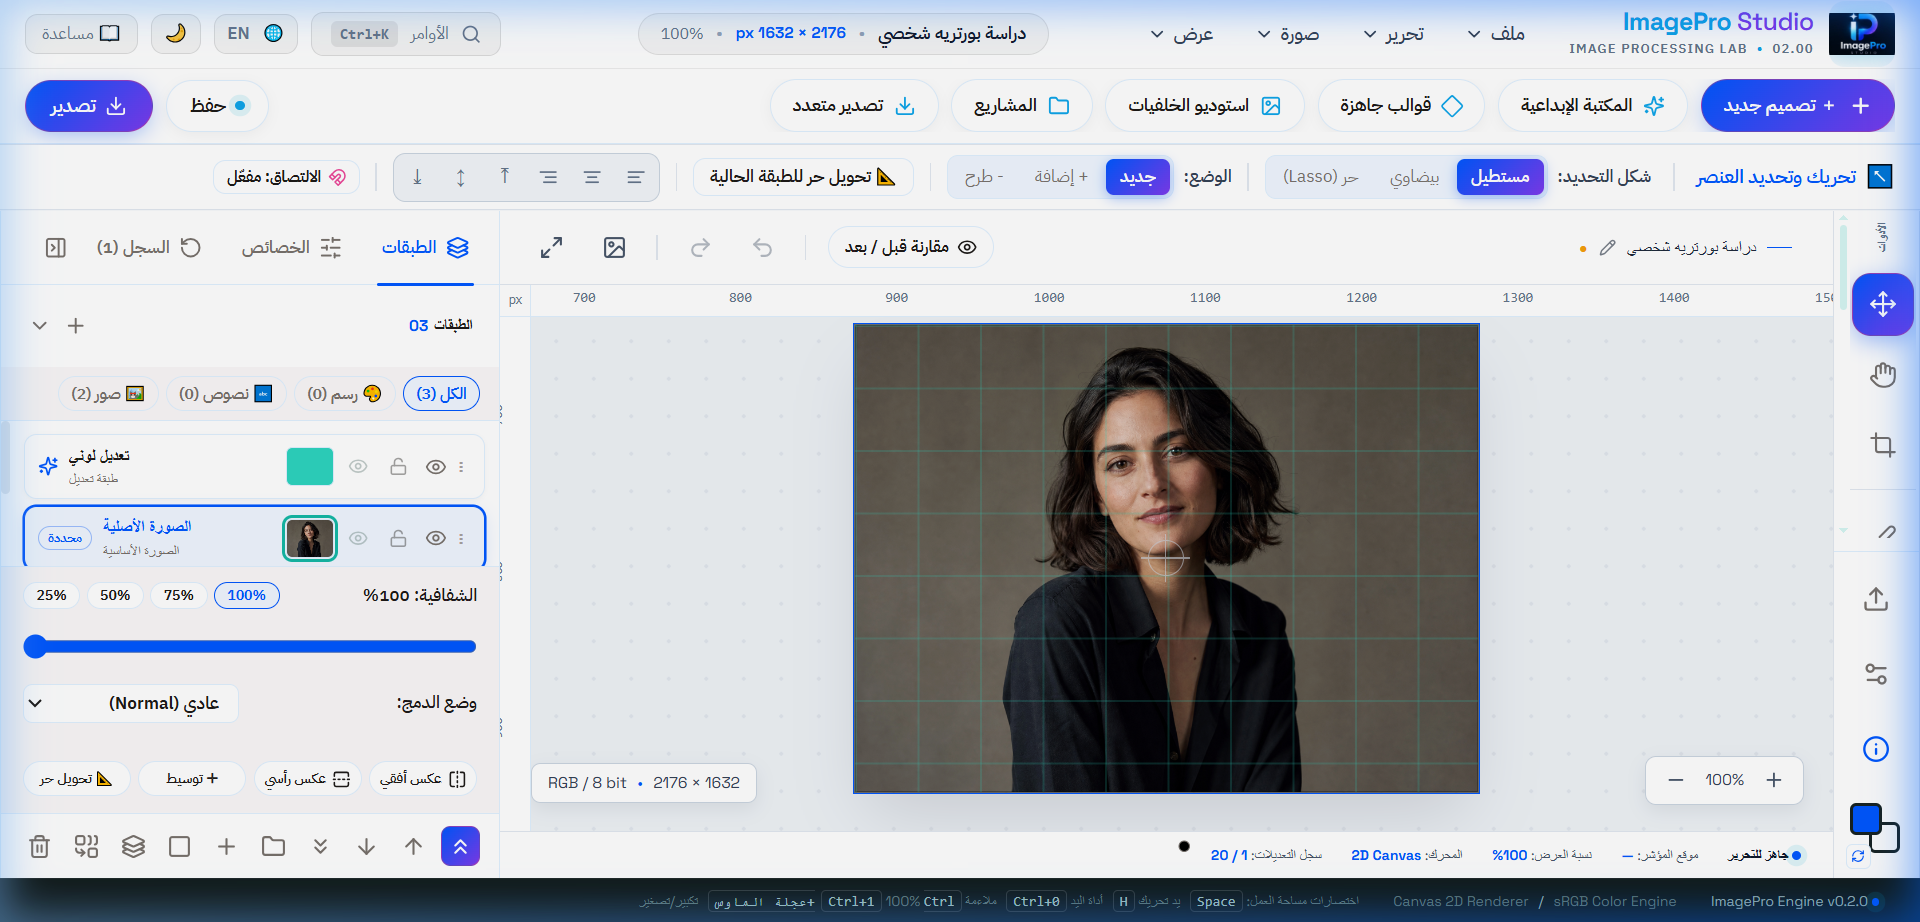
\includegraphics[width=0.96\textwidth]{01_main_workspace.png}
    \caption{الشاشة الرئيسية لنظام ImagePro Studio (الوضع الفاتح) مع الشعار الرسمي الجديد}
    \label{fig:main-workspace}
\end{figure}

\begin{techbox}{شرح تفصيلي لمكونات الشاشة الرئيسية (الشكل \ref{fig:main-workspace})}
    تتألف الشاشة الرئيسية من سبعة قطاعات وظيفية وهندسية أساسية تم تصميمها وفق معايير UX الاحترافية:
    \begin{itemize}
        \item \textbf{شعار المنصة وبطاقة الإصدار (أعلى اليمين):} أيقونة العدسة والكاميرا المحدثة بألوان الزمرد والبنفسجي، مع اسم المنصة \texttt{ImagePro Studio} وبطاقة النسخة الفنية \texttt{v3.2.0 Pro}.
        \item \textbf{شريط النظام العلوي (Tier 1 Bar):} يضم القوائم القياسية السبع: (ملف File، تعديل Edit، صورة Image، طبقة Layer، مرشحات Filter، عرض View، ومساعدة Help)، مع أزرار التراجع والإعادة (Undo/Redo)، ومؤشر الحفظ اللحظي.
        \item \textbf{شريط استوديو الإبداع (Tier 2 Hero Ribbon):} كبسولات عائمة سريعة: «＋ تصميم جديد»، «المكتبة الإبداعية»، «قوالب جاهزة»، «استوديو الخلفيات»، «المشاريع»، و«تصدير متعدد».
        \item \textbf{شريط خيارات الأداة السياقي (Contextual Tool Bar):} يتغير ديناميكياً مع كل أداة ليعرض معاييرها الخاصة (حجم الرأس، الصلابة، الشفافية، نسبة التسامح، أو الخط).
        \item \textbf{صندوق الأدوات الرأسي الأيسر (Left Toolbar):} 12 أداة هندسية متكاملة:
        \begin{enumerate}
            \item \textbf{التحريك والتحويل (Move/Transform - V):} تحريك الطبقات ومقابض التحجيم والتدوير الثمانية.
            \item \textbf{التحديد المستطيلي والبيضاوي (Marquee - M):} تحديد بكسلي هندسي منتظم.
            \item \textbf{حبل التحديد الحر (Lasso - L):} رسم مسارات تحديد يدوية ومضلعة.
            \item \textbf{العصا السحرية (Magic Wand - W):} تحديد المساحات اللونية بالمسافة الإقليدية مع نسبة التسامح.
            \item \textbf{الفرشاة الفنية (Brush - B):} رسم ناعم بانسيابية أقواس بيزيه لمنع الرعشة.
            \item \textbf{الممحاة (Eraser - E):} مسح بكسلي بصلابة وشفافية متغيرة.
            \item \textbf{سطل الطلاء (Paint Bucket - G):} ملء فيضاني للمساحات المغلقة بخوارزمية BFS.
            \item \textbf{النصوص المتجهة (Typography - T):} كتابة نصوص قابلة للتحجيم بخطوط عربية ولاتينية.
            \item \textbf{الأشكال المتجهة (Shapes - U):} رسم المستطيلات، الدوائر، النجوم، والأسهم بدقة رياضية.
            \item \textbf{القطارة اللونية (Eyedropper - I):} امتصاص لون أي بكسل ونقله للوحة الألوان.
            \item \textbf{أداة اليد (Hand - H):} تحريك مشهد العرض للتجول المريح أثناء التكبير.
            \item \textbf{التكبير والتصغير (Zoom - Z):} ضبط نسبة العرض من 10\% حتى 800\%.
        \end{enumerate}
        \item \textbf{الكانفاس والمساطر الذكية:} مسطح التصميم بدقة $2176 \times 1632$ بكسل محاط بمساطر بكسلية متدرجة وخطوط إرشادية ممغنطة للمحاذاة التلقائية (Smart Snapping).
        \item \textbf{شريط الحالة السفلي (Status Bar):} إحداثيات مؤشر الفأرة الحية $(X, Y)$، نسبة العرض، ونمط الألوان sRGB 8-bit.
    \end{itemize}
\end{techbox}

\begin{figure}[htbp]
    \centering
    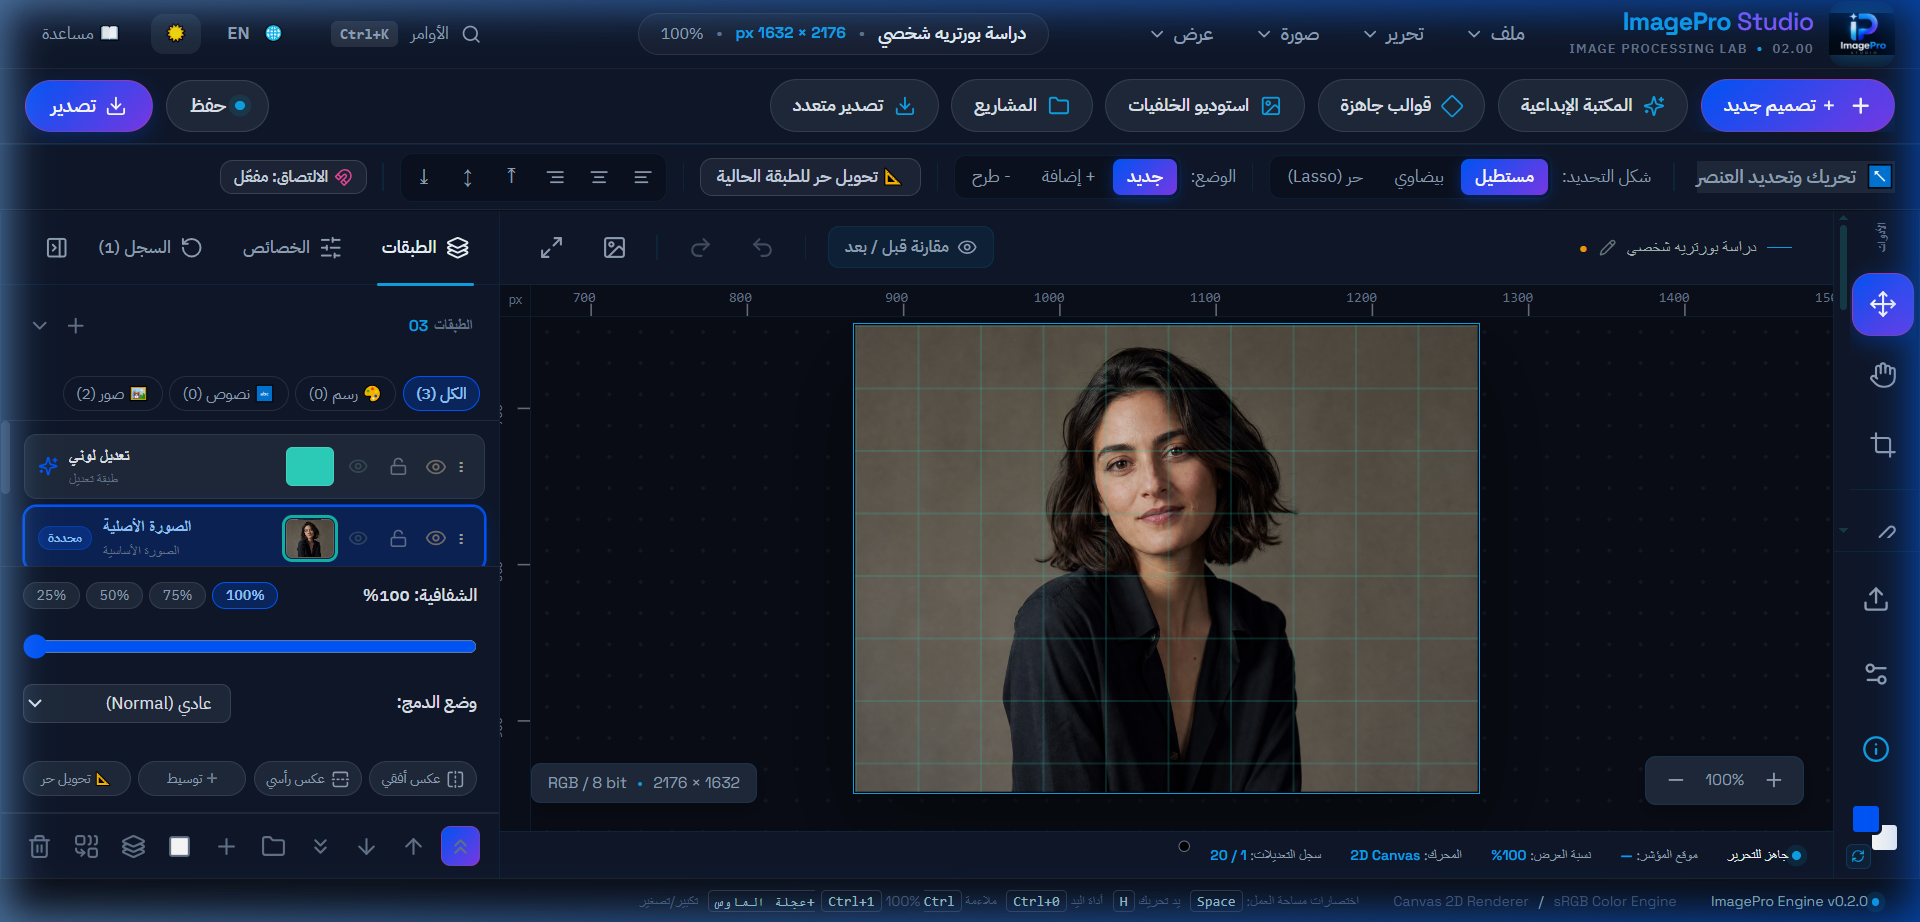
\includegraphics[width=0.96\textwidth]{02_dark_mode_workspace.png}
    \caption{مساحة العمل المحدثة بالوضع الليلي (Dark Studio Mode) مع لوحة الطبقات النشطة}
    \label{fig:dark-workspace}
\end{figure}

\begin{techbox}{شرح الوضع الليلي ولوحة الطبقات (الشكل \ref{fig:dark-workspace})}
    لقطة حية تبرز تصميم الاستوديو الداكن (\#0f172a / \#1e293b) المصمم لراحة العين وتفادي الإجهاد البصري، وتوضح بالتفصيل:
    \begin{itemize}
        \item \textbf{ترويسة لوحة الطبقات:} زر إضافة طبقة جديدة (+)، زر مضاعفة وتكرار الطبقة (Duplicate)، وزر حذف الطبقة.
        \item \textbf{قائمة أنماط المزج والدمج (17 Blending Modes):} تشمل Normal, Multiply, Screen, Overlay, Soft Light, Hard Light, Color Dodge وغيرها، وتحدد كيفية تفاعل بكسلات الطبقة رياضياً مع الطبقات السفلية.
        \item \textbf{منزلق عتامة الطبقة (Layer Opacity Slider):} تحكم مباشر بنسبة الشفافية من 0\% إلى 100\%.
        \item \textbf{عناصر التحكم بالطبقات:} معاينة مصغرة حية لكل طبقة (Live Thumbnail)، زر إظهار/إخفاء الطبقة (Eye Toggle)، قفل الطبقة (Lock Layer) لمنع التعديل العرضي، وإعادة الترتيب الرأسي عبر السحب والإفلات (Drag \& Drop Z-Index).
    \end{itemize}
\end{techbox}

\begin{figure}[htbp]
    \centering
    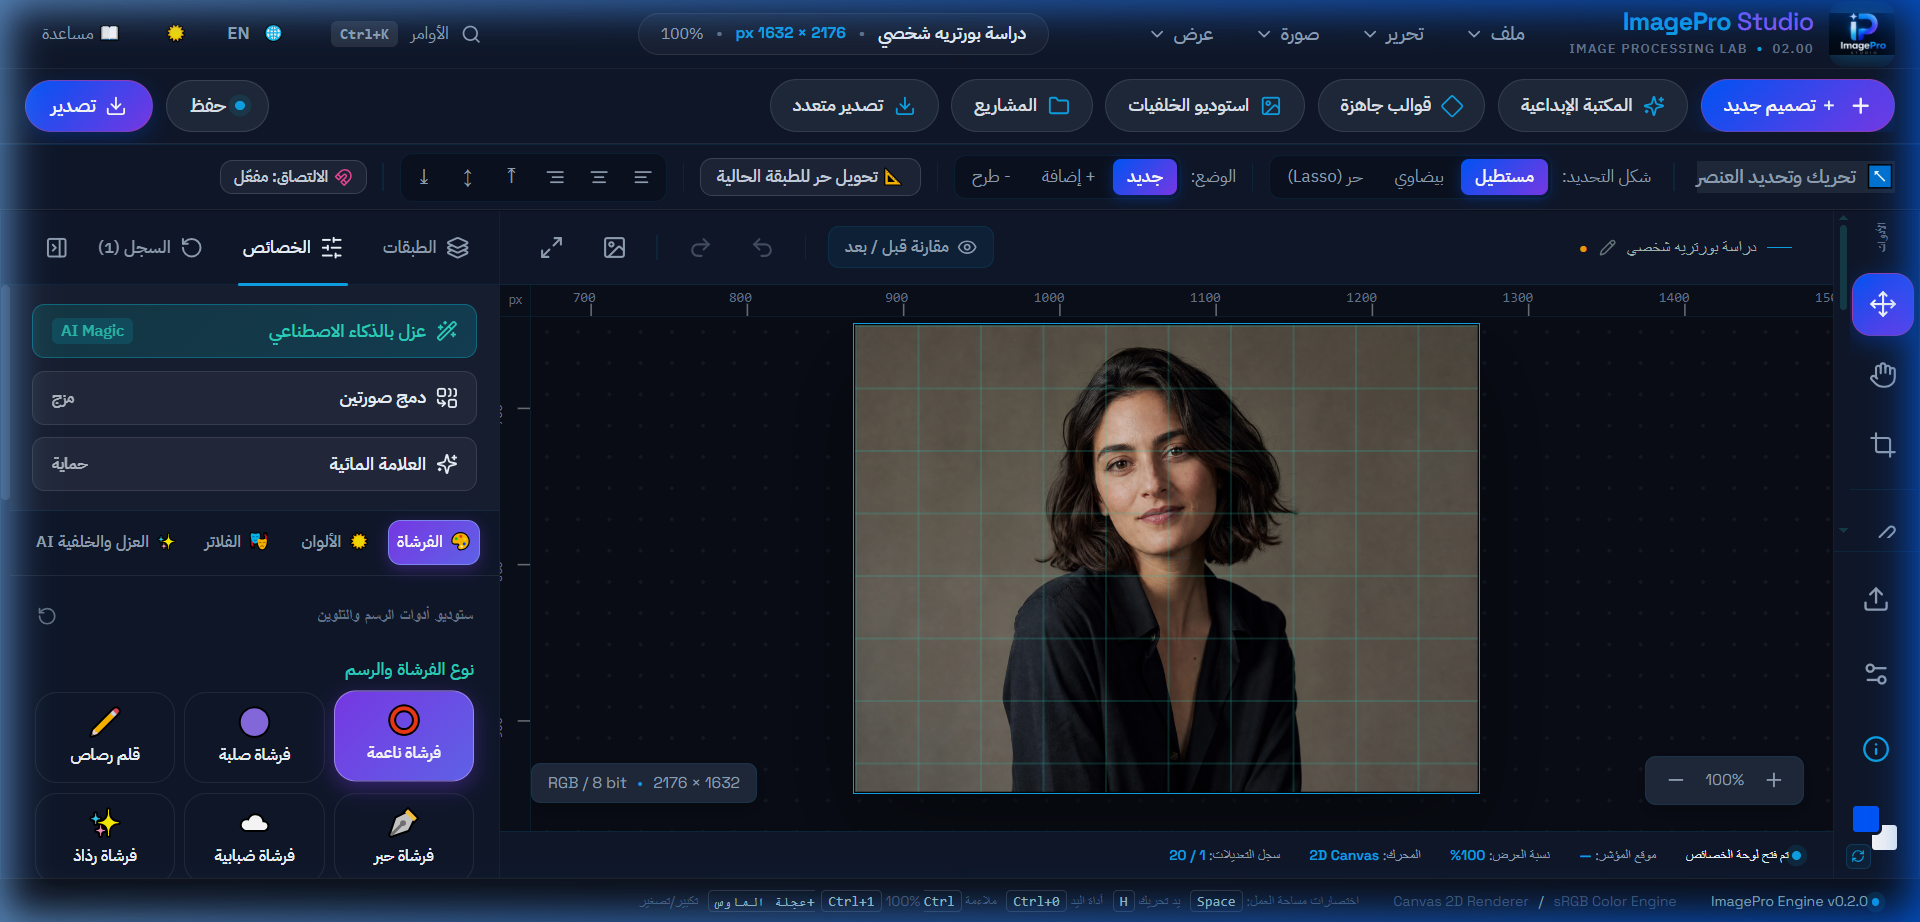
\includegraphics[width=0.96\textwidth]{04_dark_mode_properties_studio.png}
    \caption{لوحة الخصائص وأدوات الاستوديو والفرش في الوضع الليلي المحدث}
    \label{fig:dark-properties}
\end{figure}

\begin{techbox}{شرح أدوات الاستوديو والفرش في الوضع الليلي (الشكل \ref{fig:dark-properties})}
    توضح هذه اللقطة تفاصيل لوحة الخصائص الجانبية في الوضع الليلي:
    \begin{itemize}
        \item \textbf{كبسولات الاستوديو السريعة الثلاث الكبرى:}
        \begin{enumerate}
            \item \textbf{عزل بالذكاء الاصطناعي (AI Magic):} استدعاء استوديو التجزئة العصبية ونموذج IS-Net بنقرة واحدة.
            \item \textbf{دمج صورتين (Blend Images):} فتح أداة المزج المتقدم بين طبقتين بأنماط رياضية وأقنعة تدرجية.
            \item \textbf{العلامة المائية (Watermark):} استدعاء نافذة حماية الحقوق الفكرية بالنصوص والشعارات.
        \end{enumerate}
        \item \textbf{أنماط الفرشاة الجاهزة (Brush Style Presets):} فرشاة ناعمة (Soft Round) للتظليل، فرشاة صلبة (Hard Round) للتحديد الحاد، ريشة حبر (Calligraphy) لمحاكاة الخط العربي، ومرذاذ هواء (Airbrush) للرش الفني.
        \item \textbf{منزلقات التحكم الفيزيائي:} منزلق الحجم (Size من 1 إلى 200 بكسل مع معاينة دائرية حية)، منزلق صلابة الحواف (Hardness \%)، ومنزلق العتامة والتدفق (Opacity \%).
    \end{itemize}
\end{techbox}

\newpage
\section{شريط استوديو الإبداع (Tier 2 Hero Ribbon)}

\begin{figure}[htbp]
    \centering
    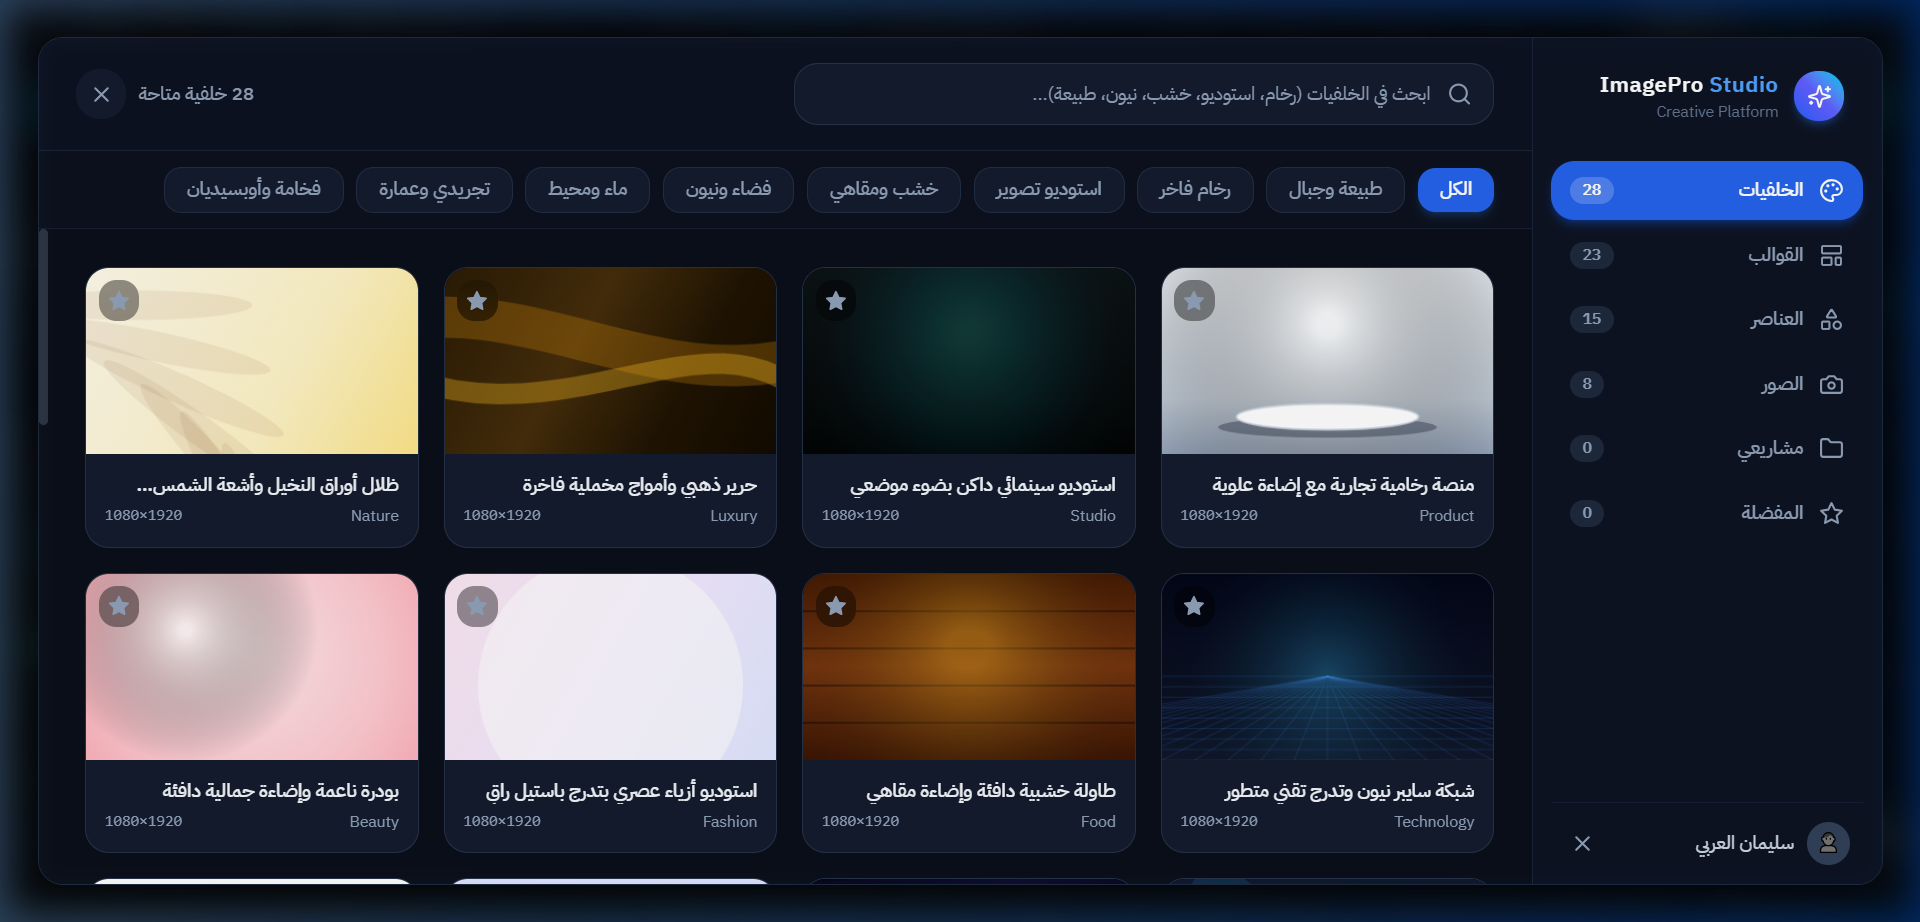
\includegraphics[width=0.95\textwidth]{03_hero_ribbon.png}
    \caption{شريط استوديو الإبداع الموحد (Tier 2 Hero Ribbon)}
    \label{fig:hero-ribbon}
\end{figure}

\begin{techbox}{تفصيل كبسولات شريط الإبداع (الشكل \ref{fig:hero-ribbon})}
    شريط كبسولي عائم يختصر تدفق العمل الإنتاجي عبر أزرار الوصول الفوري:
    \begin{itemize}
        \item \textbf{زر «＋ تصميم جديد»:} تهيئة مشروع جديد بالمقاسات الجاهزة للسوشيال ميديا أو الطباعة أو بالأبعاد المخصصة.
        \item \textbf{المكتبة الإبداعية:} مستودع يضم آلاف الأصول المتجهة وصور الستوك والملصقات القابلة للإفلات المباشر على الكانفاس.
        \item \textbf{قوالب جاهزة:} تصفح مئات القوالب المصممة الجاهزة للتحرير بكامل طبقاتها المستقلة.
        \item \textbf{استوديو الخلفيات:} تصوير المنتجات، المنصات ثلاثية الأبعاد (Podiums)، وتدرجات استوديو البورتريه.
        \item \textbf{المشاريع:} إدارة المشاريع المحفوظة محلياً في IndexedDB وسجل النسخ الاحتياطية وسلة المهملات.
        \item \textbf{تصدير متعدد:} توليد وتصدير كافة مقاسات منصات التواصل الاجتماعي دفعة واحدة داخل ملف ZIP.
    \end{itemize}
\end{techbox}

\section{لوحة الأوامر السريعة (Command Palette)}

\begin{figure}[htbp]
    \centering
    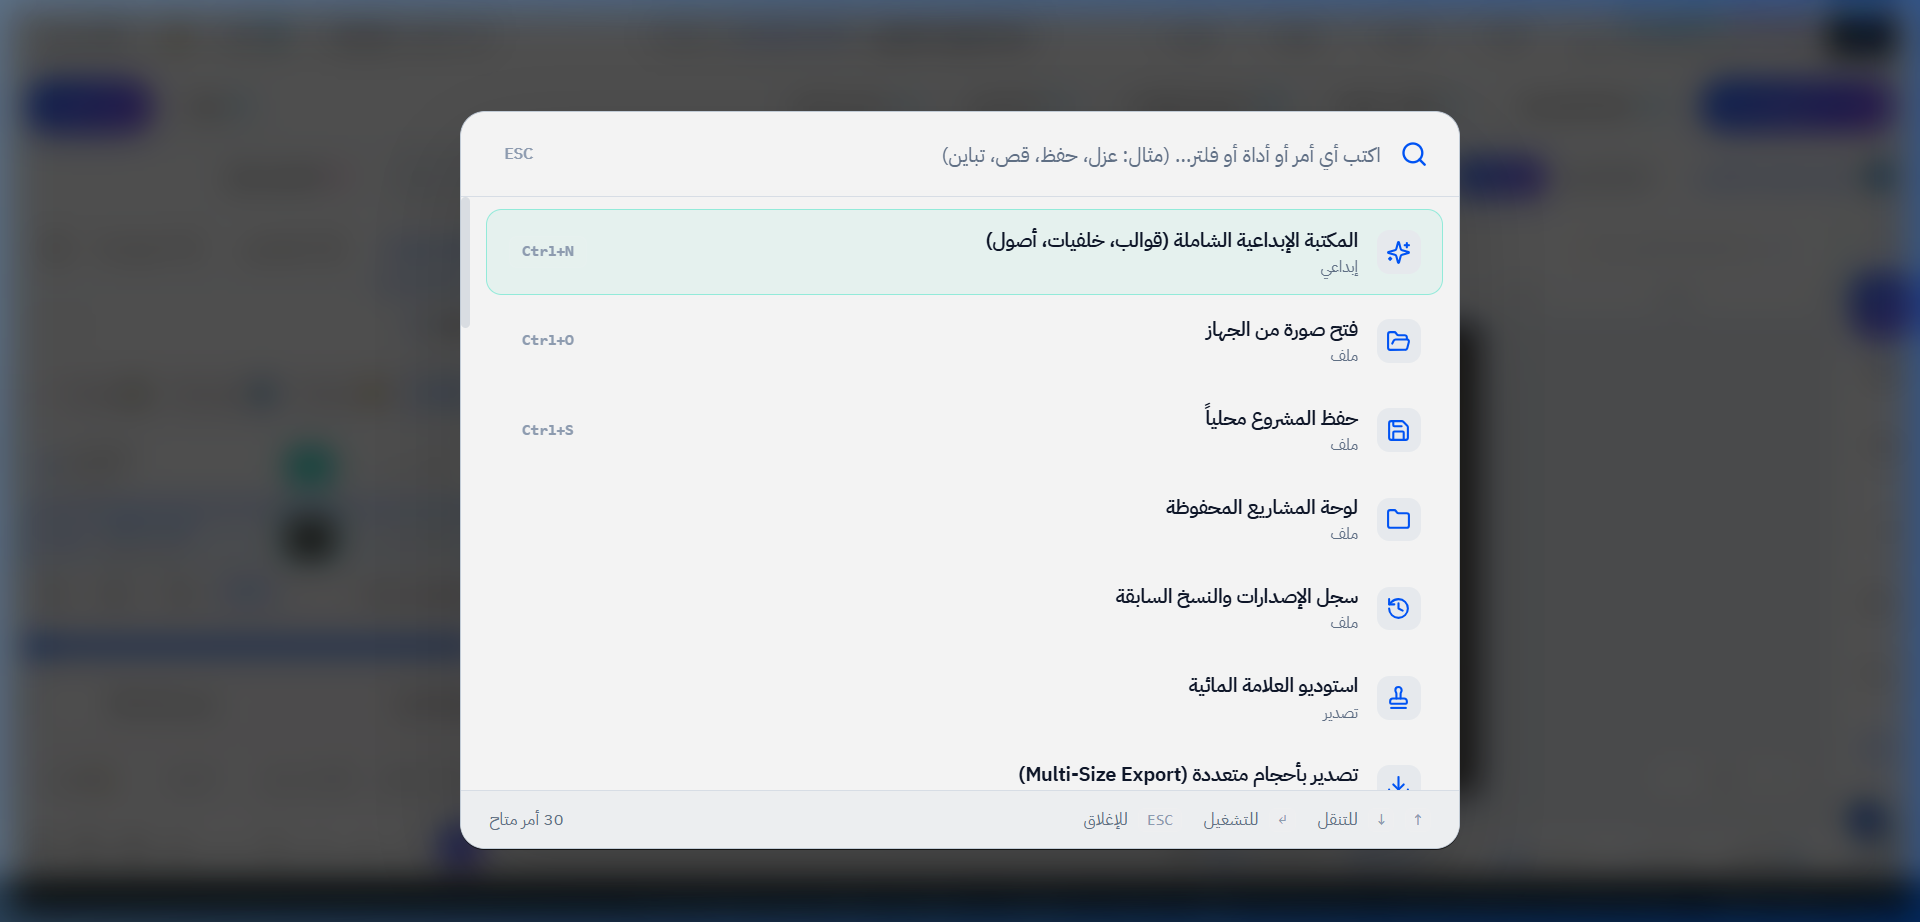
\includegraphics[width=0.85\textwidth]{20_command_palette.png}
    \caption{لوحة الأوامر السريعة الفورية (Command Palette -- \texttt{Ctrl + K})}
    \label{fig:command-palette}
\end{figure}

\begin{techbox}{شرح لوحة الأوامر ومحرك البحث (الشكل \ref{fig:command-palette})}
    واجهة تحكم فورية مستوحاة من أحدث بيئات التصميم المتقدمة:
    \begin{itemize}
        \item \textbf{محرك المطابقة التقريبية (Fuzzy Matching Engine):} يتيح العثور على الأوامر حتى مع الأخطاء الإملائية الطفيفة.
        \item \textbf{التصنيف الهيكلي للنتائج:} تصنيف الأوامر إلى: أدوات التصميم (Tools)، الفلاتر والمؤثرات (Filters)، النوافذ المنبثقة (Modals)، وعمليات التصدير والحفظ (Actions).
        \item \textbf{بطاقات الاختصارات (Shortcuts Badges):} إظهار اختصار لوحة المفاتيح المقابل لكل أمر بجانبه مباشرة (مثل \texttt{B} للفرشاة، \texttt{Ctrl+Z} للتراجع).
        \item \textbf{التنفيذ من لوحة المفاتيح:} التنقل بأسهم الكيبورد والضغط على \texttt{Enter} لتنفيذ الأمر فوراً دون لمس الفأرة.
    \end{itemize}
\end{techbox}

% ═════════════════════════════════════════════════════════════════════
% الفصل الخامس: النوافذ الإبداعية والاستوديوهات المتخصصة
% ═════════════════════════════════════════════════════════════════════
\chapter{النوافذ الإبداعية والاستوديوهات المتخصصة}

\section{نافذة بدء التصميم والمقاسات الجاهزة}

\begin{figure}[htbp]
    \centering
    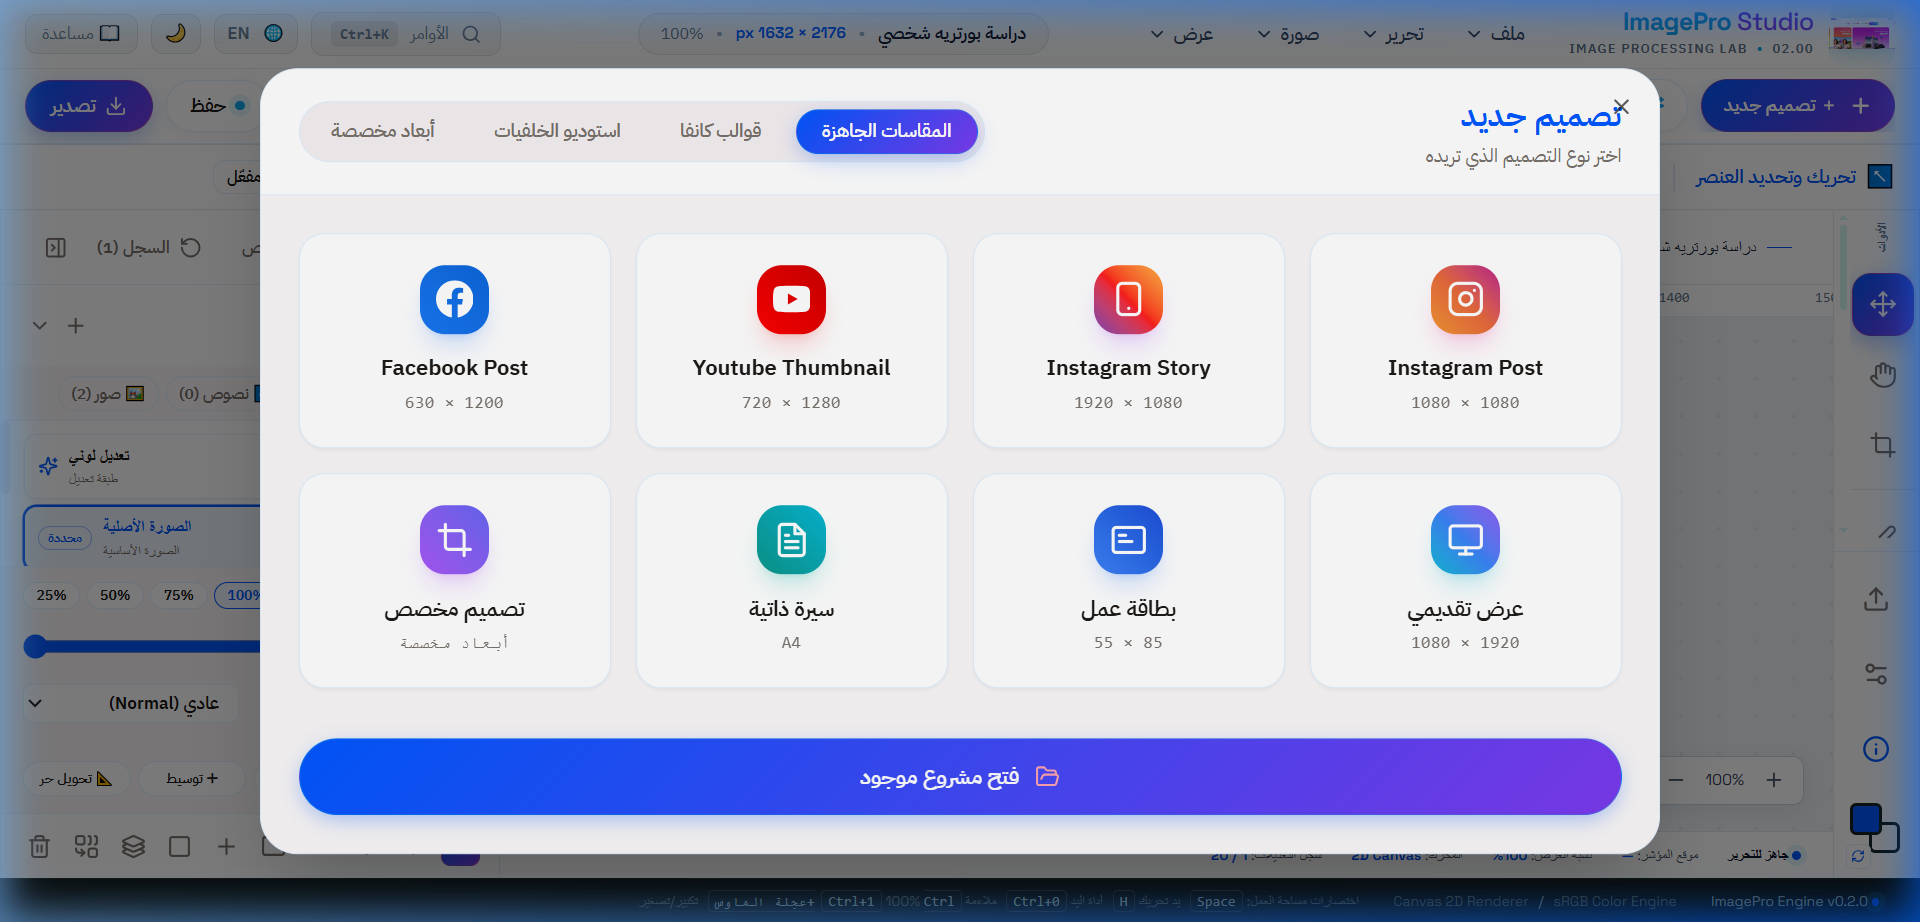
\includegraphics[width=0.90\textwidth]{05_new_design_modal.png}
    \caption{نافذة «تصميم جديد» بمقاسات السوشيال ميديا والطباعة والأبعاد المخصصة}
    \label{fig:new-design-modal}
\end{figure}

\begin{techbox}{تفصيل خيارات ومقاسات نافذة التصميم الجديد (الشكل \ref{fig:new-design-modal})}
    واجهة مخصصة لتهيئة الأعمال الفنية الجديدة وفق المعايير القياسية العالمية:
    \begin{itemize}
        \item \textbf{تبويب مقاسات السوشيال ميديا (Social Media):}
        \begin{itemize}
            \item بوست فيسبوك ($1200 \times 630$ بكسل).
            \item بوست انستغرام المربع ($1080 \times 1080$ بكسل).
            \item قصة وريلز انستغرام وتيك توك ($1080 \times 1920$ بكسل).
            \item صورة مصغرة يوتيوب YouTube Thumbnail ($1280 \times 720$ بكسل).
            \item غلاف منصة تويتر/إكس Header ($1500 \times 500$ بكسل).
        \end{itemize}
        \item \textbf{تبويب المطبوعات والأعمال (Print \& Business):}
        \begin{itemize}
            \item مستند A4 طباعي ($2480 \times 3508$ بكسل بدقة 300 DPI).
            \item بطاقة عمل شخصية Business Card ($1050 \times 600$ بكسل).
            \item ملصق إعلاني Poster A3 ($3508 \times 4960$ بكسل).
        \end{itemize}
        \item \textbf{قسم الأبعاد المخصصة (Custom Dimensions):} حقول إدخال العرض (Width) والارتفاع (Height) بالبكسل، مع زر قفل نسبة التناسب لمنع تشوه الأبعاد.
        \item \textbf{محدد لون خلفية الكانفاس الافتراضية:} شفاف (Transparent Checkerboard)، أبيض نقي، أسود استوديو، أو لون مخصص عبر منتقي الألوان.
        \item \textbf{زر الإجراء النهائي:} زر «إنشاء مساحة العمل» الذي يقوم بتهيئة الكانفاس، وتفعيل طبقة الخلفية، وضبط المساطر الذكية تلقائياً.
    \end{itemize}
\end{techbox}

\section{المكتبة الإبداعية الشاملة للأصول (Creative Library Hub)}

\begin{figure}[htbp]
    \centering
    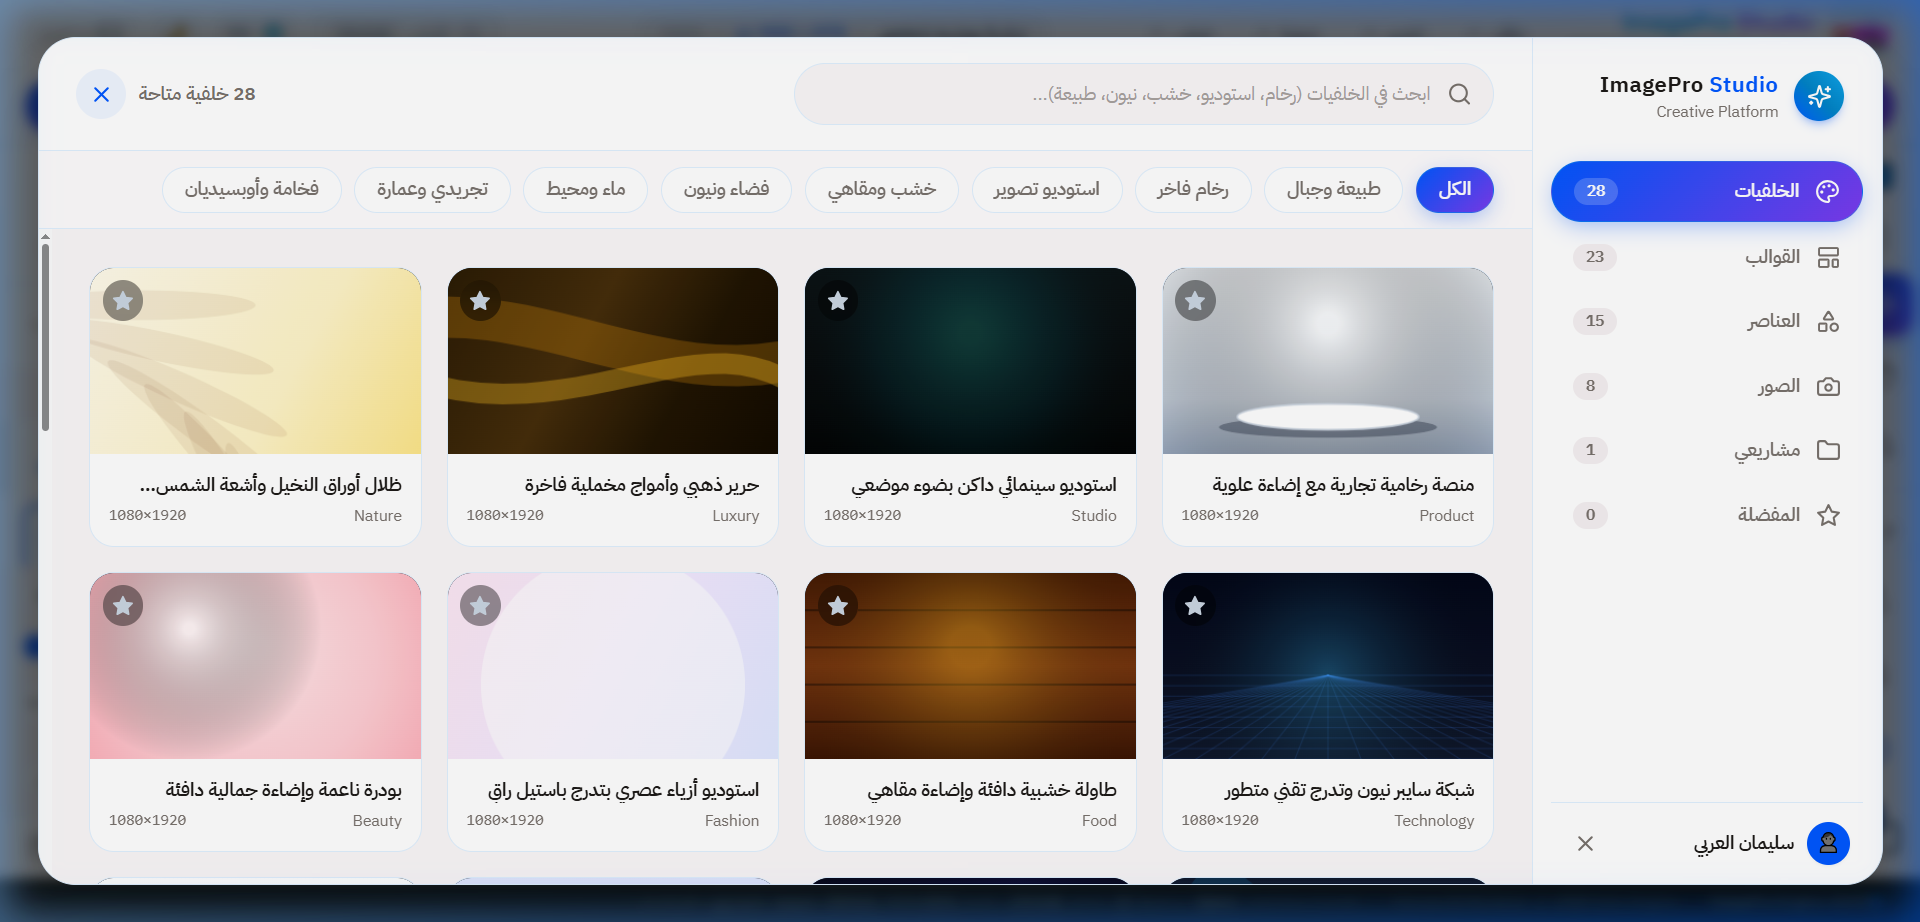
\includegraphics[width=0.90\textwidth]{06_creative_library_modal.png}
    \caption{المكتبة الإبداعية الشاملة للأصول المتجهة، الصور، والملصقات}
    \label{fig:creative-library}
\end{figure}

\begin{techbox}{محتويات وأقسام المكتبة الإبداعية (الشكل \ref{fig:creative-library})}
    مستودع أصول تصميم رقمية متكامل يضم آلاف العناصر المصنفة:
    \begin{itemize}
        \item \textbf{قسم الرسومات المتجهة (Vector Elements):} مئات الرموز والأشكال التجريدية المرسومة برمجياً بدوال \texttt{Canvas 2D Path} النقية دون الحاجة لملفات صور ثقيلة، مما يضمن دقة لانهائية وسرعة فائقة.
        \item \textbf{مستودع صور الستوك الفوتوغرافية (Stock Photos Hub):} صور فوتوغرافية احترافية عالية الدقة مصنفة حسب المجالات (الطبيعة، التكنولوجيا، الأعمال، البورتريه، والأطعمة).
        \item \textbf{الملصقات والشارات الترويجية (Stickers \& Badges):} شرائط الخصومات، أختام الجودة، والنجوم التقييمية الجاهزة للإعلانات التجارية.
        \item \textbf{محرك السحب والإفلات الذكي (Smart Drag \& Drop Hub):} دعم سحب أي عنصر من النافذة وإفلاته في أي نقطة على الكانفاس ليقوم النظام فوراً بإنشاء طبقة جديدة متموضعة في نفس إحداثيات الإفلات.
    \end{itemize}
\end{techbox}

\section{استوديو القوالب الجاهزة متعددة الطبقات}

\begin{figure}[htbp]
    \centering
    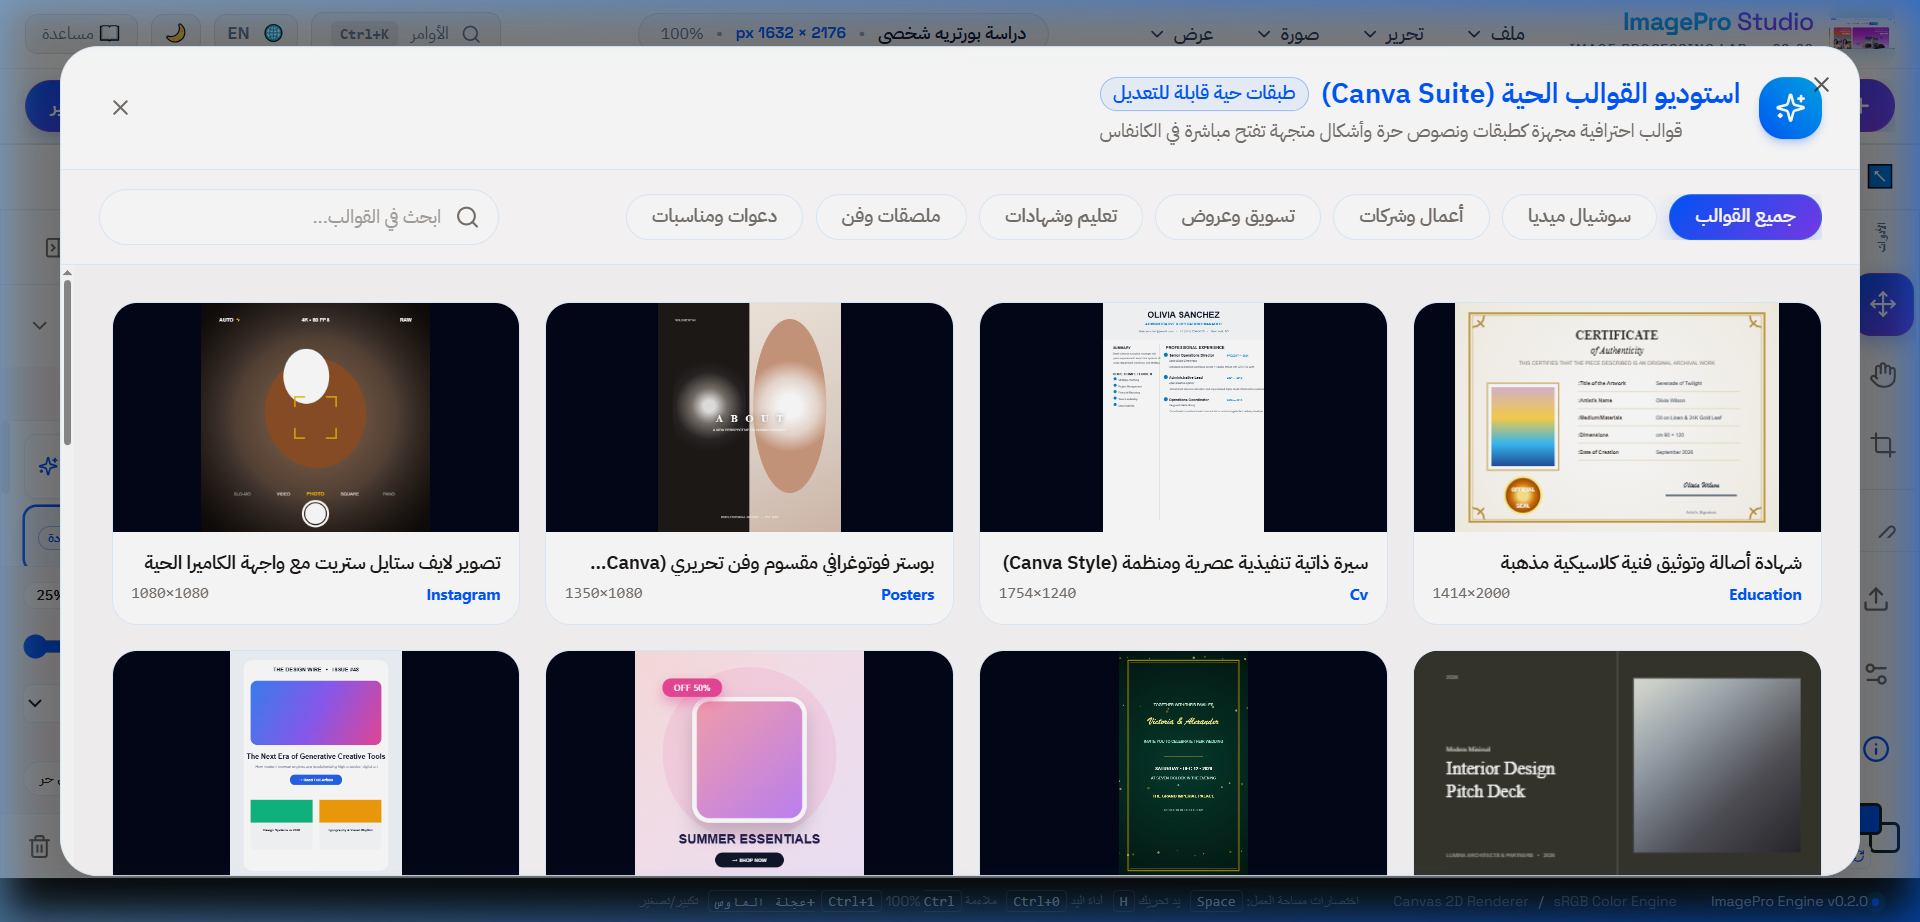
\includegraphics[width=0.90\textwidth]{07_templates_modal.png}
    \caption{استوديو القوالب الجاهزة القابلة للتحرير بجميع طبقاتها}
    \label{fig:templates-modal}
\end{figure}

\begin{techbox}{بنية القوالب وتدفق العمل الهيكلي (الشكل \ref{fig:templates-modal})}
    بيئة لاستعراض واختيار القوالب التصميمية الجاهزة والمعدة بأعلى معايير الجماليات البصرية:
    \begin{itemize}
        \item \textbf{التصنيفات الوظيفية للقوالب:} قوالب عروض التجارة الإلكترونية، إعلانات المطاعم، منشورات السوشيال ميديا، وبطاقات الأعمال والمناسبات.
        \item \textbf{تفكيك القالب إلى طبقات مستقلة (Layer Decomposition):} عند اختيار أي قالب، لا يتم تنزيله كصورة مسطحة بل يقوم النظام ببناء شجرة طبقات كاملة في الكانفاس تشمل: طبقة الصورة الخلفية، طبقات الكتل اللونية المتجهة، طبقات النصوص القابلة للتحرير المباشر بالخطوط العربية والأجنبية، وشارات الأسعار والشعارات.
        \item \textbf{مزامنة الخطوط التلقائية:} تحميل خطوط القالب وتطبيقها لحظياً على النصوص دون فقدان التنسيق الجمالي.
    \end{itemize}
\end{techbox}

\section{استوديو الخلفيات وتصوير المنتجات والبورتريه}

\begin{figure}[htbp]
    \centering
    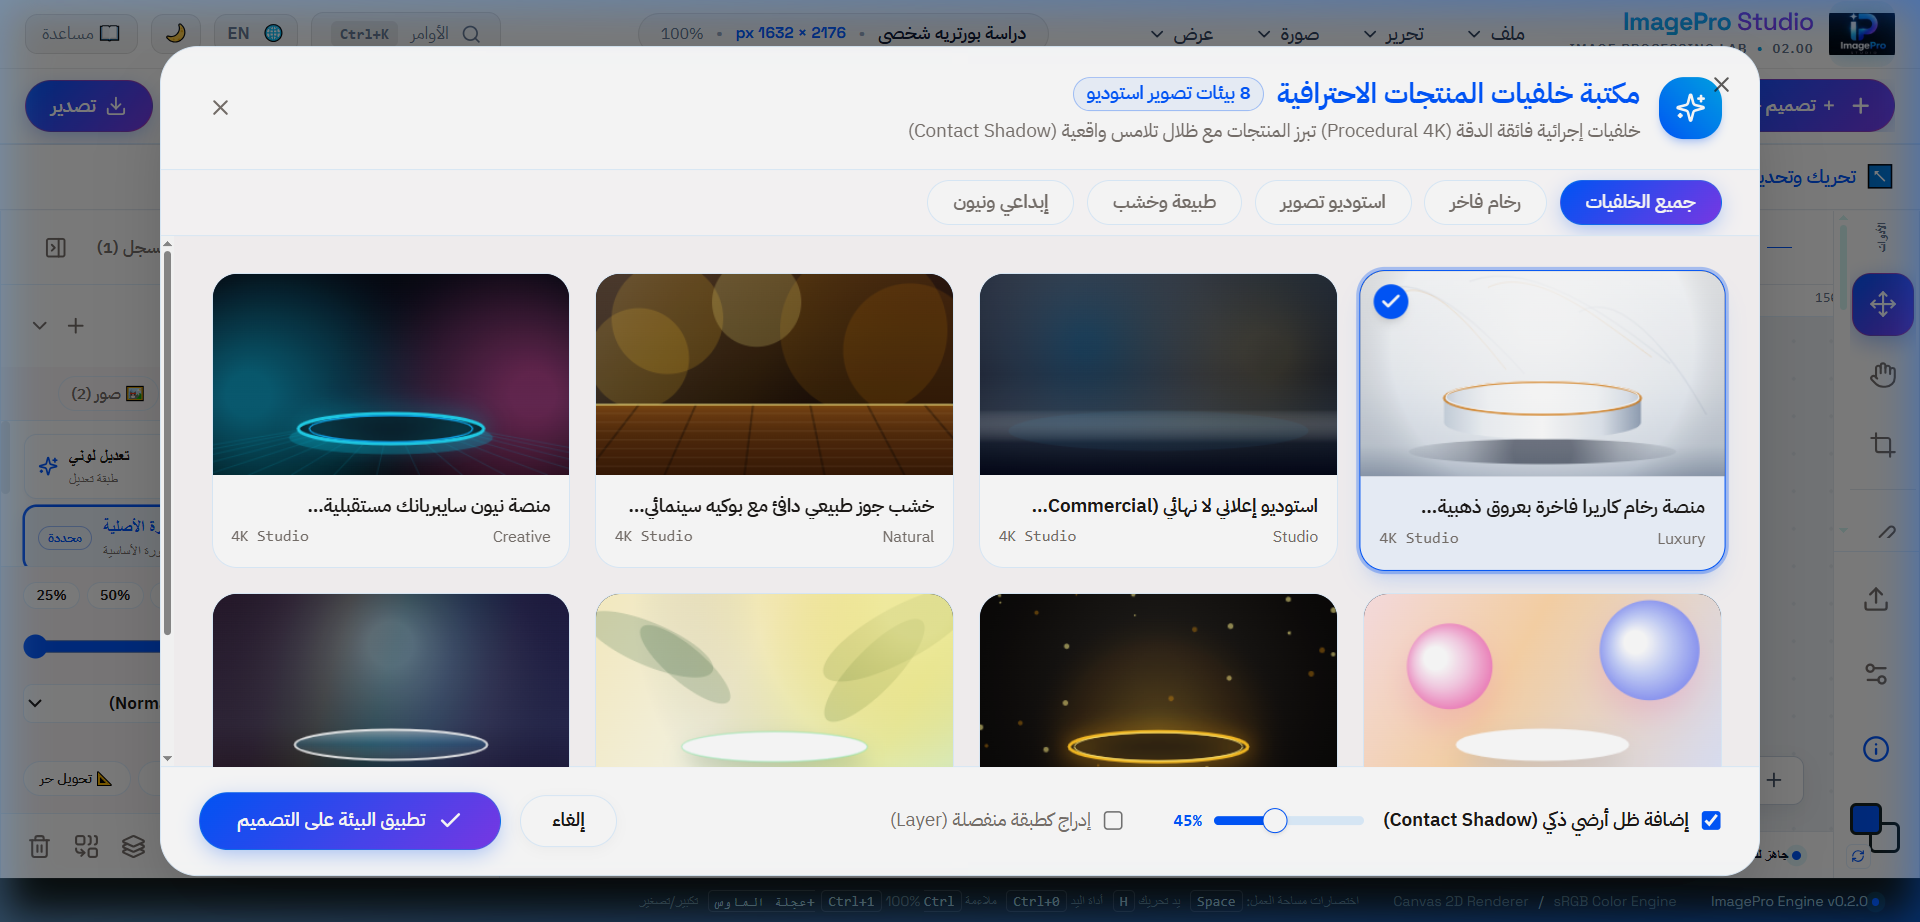
\includegraphics[width=0.90\textwidth]{08_backdrops_modal.png}
    \caption{استوديو الخلفيات لتصوير المنتجات، المنصات، والتدرجات البورتريه}
    \label{fig:backdrops-modal}
\end{figure}

\begin{techbox}{تفصيل فئات الخلفيات في الاستوديو (الشكل \ref{fig:backdrops-modal})}
    مكتبة متخصصة موجهة لمصممي المتاجر الإلكترونية والإعلانات التجارية:
    \begin{itemize}
        \item \textbf{فئة المنصات والبوديوم (3D Podiums \& Pedestals):} منصات رخامية دائرية ومستطيلة، منصات إسمنتية عصرية، ومنصات خشبية دافئة مع ظلال وإضاءات واقعية لعرض المنتجات فوقها.
        \item \textbf{فئة إضاءة الاستوديو وتدرجات البورتريه (Studio Lighting Spots):} بقع ضوئية وتدرجات فينيل سينمائية تمنح صور البورتريه فخامة وعمقاً بصرياً.
        \item \textbf{فئة الطبيعة والباستيل (Nature \& Pastel Backdrops):} ظلال أوراق الشجر الناعمة، تدرجات الشروق والغروب الهادئة، وأسطح الرمال الذهبية.
        \item \textbf{تطبيق الخلفية التلقائي:} إمكانية إدراج الخلفية مباشرة أسفل عناصر التصميم المعزولة لتكوين مشهد تجاري متكامل في ثوانٍ معدودة.
    \end{itemize}
\end{techbox}

\section{لوحة إدارة المشاريع وسجل النسخ (Projects Dashboard)}

\begin{figure}[htbp]
    \centering
    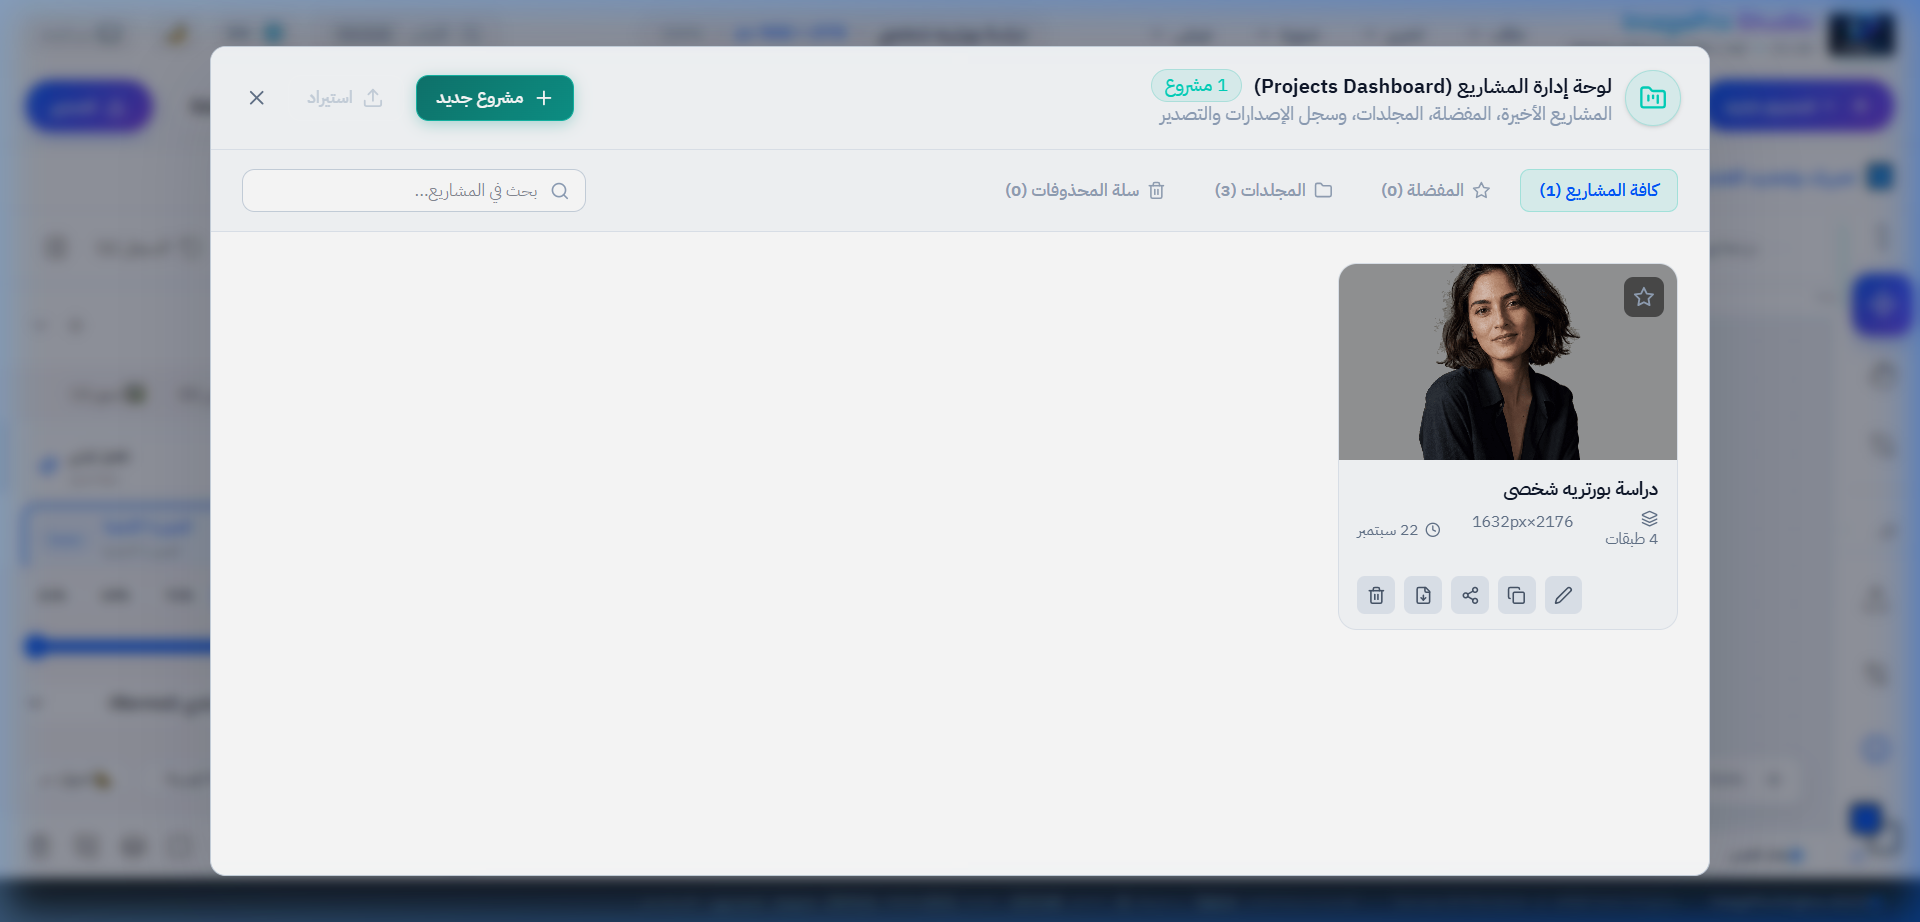
\includegraphics[width=0.88\textwidth]{16_projects_dashboard.png}
    \caption{لوحة إدارة المشاريع المحفوظة محلياً وسجل النسخ وسلة المهملات}
    \label{fig:projects-dashboard}
\end{figure}

\begin{techbox}{مكونات وخصائص لوحة إدارة المشاريع (الشكل \ref{fig:projects-dashboard})}
    نظام محلي متكامل لإدارة المشاريع الفنية يعتمد على التخزين الهجين بين \texttt{IndexedDB} للبيانات الضخمة و \texttt{localStorage} للإعدادات الوصفية:
    \begin{itemize}
        \item \textbf{بطاقات المشاريع المحفوظة (Project Cards):} تعرض كل بطاقة مصغراً حقيقياً للعمل الفني، اسم المشروع، تاريخ ووقت آخر تعديل، أبعاد الكانفاس، وحجم البيانات في الذاكرة.
        \item \textbf{زر فتح واستئناف العمل (Open Project):} إعادة تحميل كامل طبقات المشروع وإعداداته في الكانفاس واستئناف التحرير فوراً.
        \item \textbf{زر تكرار المشروع (Duplicate Project):} إنشاء نسخة مطابقة من المشروع لاختبار تصاميم بديلة دون التأثير على العمل الأصلي.
        \item \textbf{زر النقل إلى سلة المهملات (Move to Trash):} حذف آمن ينقل المشروع إلى سلة المحذوفات المؤقتة لمنع الحذف العرضي.
        \item \textbf{تبويب سلة المحذوفات (Trash Hub):} إمكانية استعراض المشاريع المحذوفة مع خيار «استعادة» فوري يعيد المشروع لمكانه، أو خيار «حذف نهائي» لتفريغ سعة التخزين.
    \end{itemize}
\end{techbox}

% ═════════════════════════════════════════════════════════════════════
% الفصل السادس: محركات المعالجة البكسلية والرياضية
% ═════════════════════════════════════════════════════════════════════
\chapter{محركات المعالجة البكسلية والرياضية}

\section{استوديو الفلاتر والالتفاف الرياضي (2D Convolution)}

\begin{figure}[htbp]
    \centering
    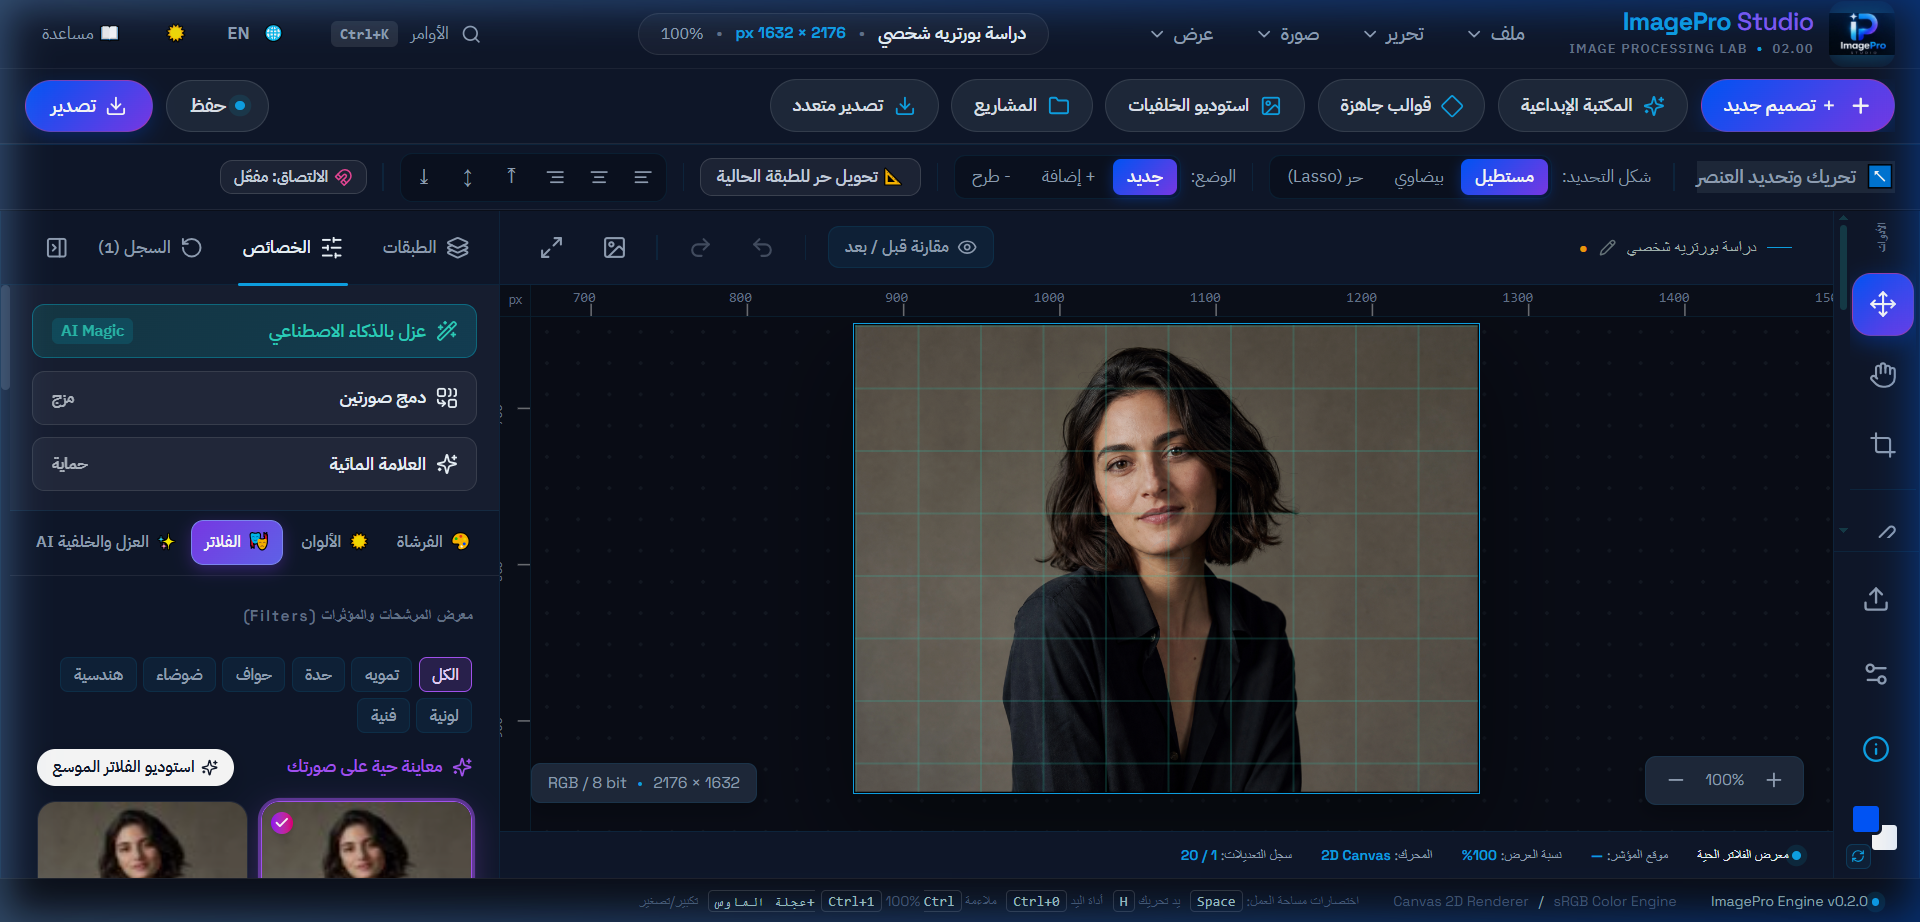
\includegraphics[width=0.85\textwidth]{09_filters_studio.png}
    \caption{لوحة استوديو الفلاتر الـ 21 مع المعاينات الحية المصغرة}
    \label{fig:filters-studio}
\end{figure}

\begin{techbox}{تفصيل واجهة استوديو الفلاتر والأسس الرياضية (الشكل \ref{fig:filters-studio})}
    لقطة حية من التحديث الأخير توضح استوديو الفلاتر بتصميمه الأزرق والبنفسجي الأنيق:
    \begin{itemize}
        \item \textbf{ترويسة اللوحة (Filters Header):} أيقونة المرشحات مع عنوان «استوديو الفلاتر» وزر الإغلاق وزر إعادة ضبط التأثيرات.
        \item \textbf{مجموعات الفلاتر الـ 21 المصنفة:}
        \begin{enumerate}
            \item \textbf{فلاتر التمويه والتنعيم:} التمويه الغوسي (Gaussian Blur)، التمويه الصندوقي (Box Blur)، تمويه الحركة (Motion Blur).
            \item \textbf{فلاتر كشف الحواف والهندسة:} كاشف سوبل الأفقي والعمودي (Sobel)، كاشف كاندي متعدد المراحل (Canny Edge)، ومرشح لابلارسيان (Laplacian).
            \item \textbf{فلاتر التوضيح والحدة:} قناع التوضيح غير الحاد (Unsharp Masking)، مرشح التمرير العالي (High Pass Sharpen).
            \item \textbf{فلاتر المؤثرات الفنية والتشويه:} مرشح التجسيم ثلاثي الأبعاد (3D Emboss)، مرشح الرسم الزيتي (Oil Painting)، ومرشح البكسلة والفسيفساء (Pixelate Mosaic).
        \end{enumerate}
        \item \textbf{بطاقات المعاينة المصغرة الحية (Interactive Live Thumbnails):} توليد مصغر مستقل لكل فلتر يعرض المعاينة المباشرة لتأثيره على صورة المشروع في الوقت الفعلي.
        \item \textbf{منزلقات التحكم التفاعلي:} منزلق قوة الفلتر (Intensity \%) من 0\% إلى 100\%، ومنزلق نصف قطر النواة (Kernel Radius / Size) لتحديد أبعاد مصفوفة الالتفاف ($3 \times 3$ أو $5 \times 5$).
        \item \textbf{الأساس الرياضي للالتفاف ثنائي الأبعاد (2D Spatial Convolution):}
        \begin{equation}
            I'(x, y) = \sum_{i=-k}^{k} \sum_{j=-k}^{k} I(x+i, y+j) \cdot K(i, j)
        \end{equation}
        وفي كاشف سوبل يتم احتساب مقدار التدرج عبر المشتقات الأفقية والعمودية: $|G| = \sqrt{G_x^2 + G_y^2}$.
    \end{itemize}
\end{techbox}

\section{محرك التعديلات الضوئية والمدرج التكراري الحي (Live Histogram)}

\begin{figure}[htbp]
    \centering
    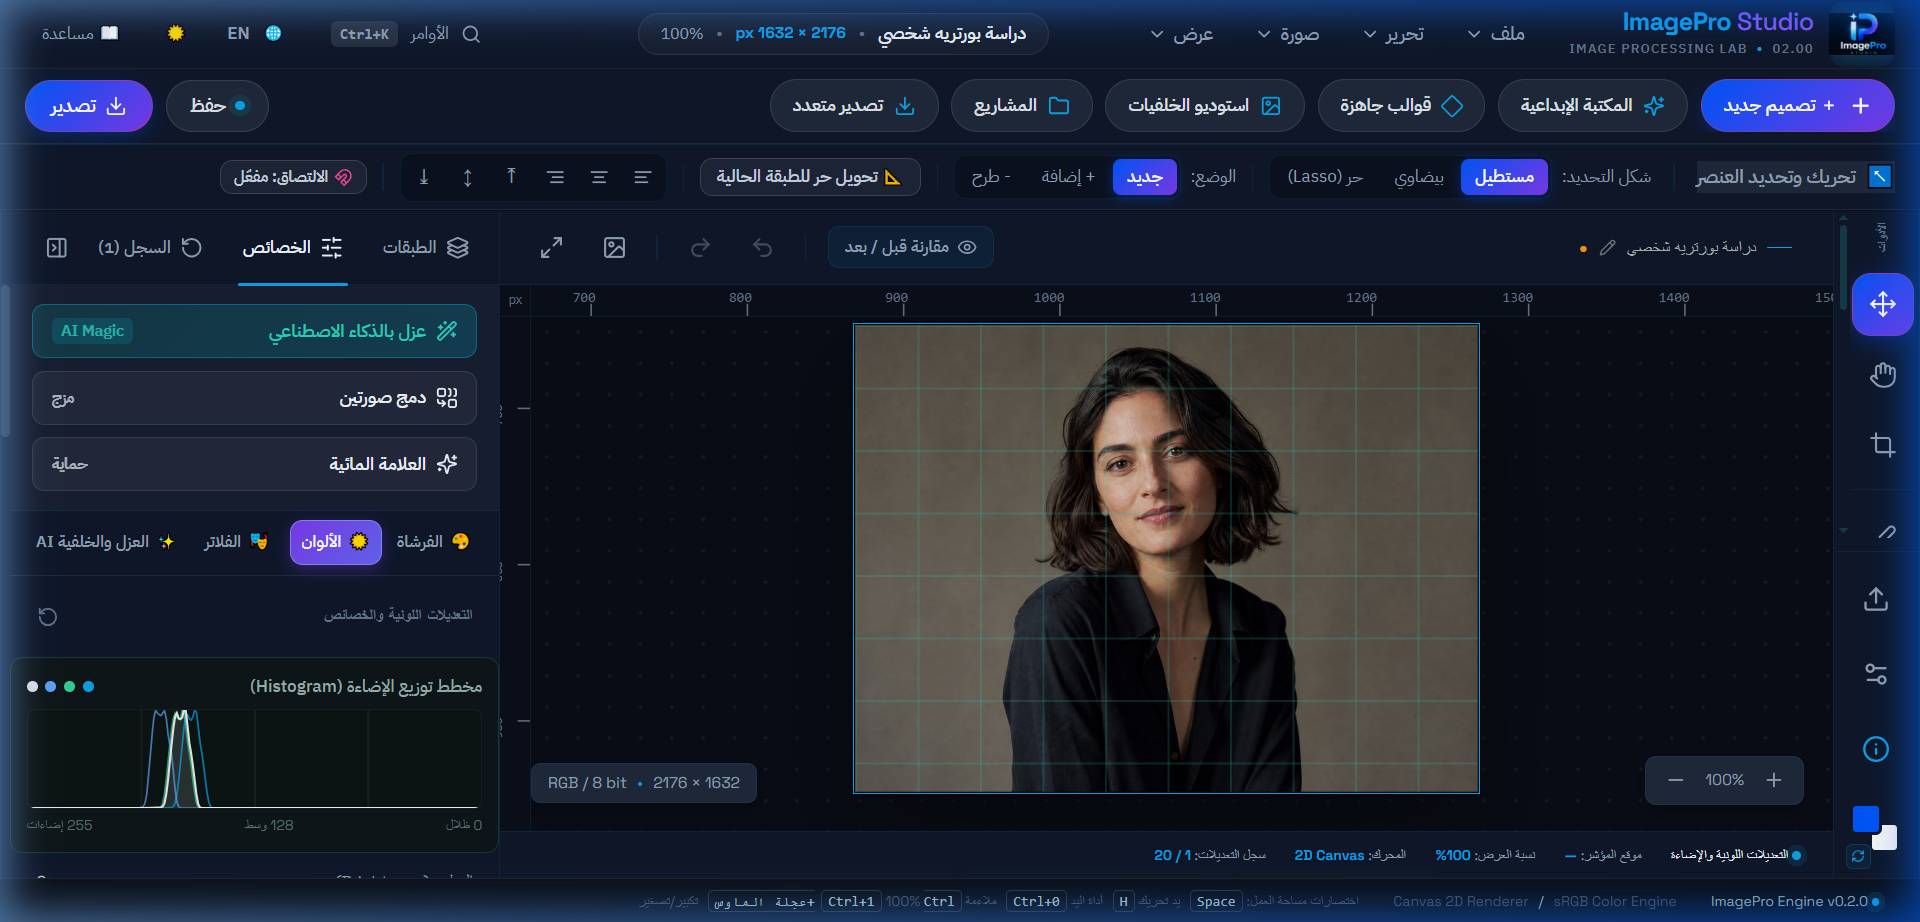
\includegraphics[width=0.85\textwidth]{10_color_adjustments_histogram.png}
    \caption{لوحة التعديلات اللونية والمدرج التكراري اللحظي (RGB Histogram) -- التحديث الأخير}
    \label{fig:color-adjustments}
\end{figure}

\begin{techbox}{تفصيل لوحة الألوان والهستوجرام والمعادلات الرياضية (الشكل \ref{fig:color-adjustments})}
    لقطة حية من التحديث الأخير توضح واجهة المعايرة الضوئية الاحترافية:
    \begin{itemize}
        \item \textbf{المدرج التكراري اللحظي المتراكب (Live Dynamic Histogram):}
        \begin{itemize}
            \item يمثل المحور الأفقي 256 مستوى شدة ضوئية (0 للظلال، 128 للوسط، 255 للإضاءات القصوى).
            \item يعرض المنحنيات اللونية للقنوات الأربع: الأحمر (Red)، الأخضر (Green)، الأزرق (Blue)، وقناة الإضاءة الإجمالية (Luminance).
            \item يحسب بمسح أحادي فائق السرعة $O(N)$ لمصفوفة البكسلات.
        \end{itemize}
        \item \textbf{منزلقات الضبط الضوئي الدقيق:}
        \begin{itemize}
            \item \textbf{السطوع (Brightness):} إزاحة خطية لمستويات الإضاءة من $-100$ إلى $+100$.
            \item \textbf{التباين (Contrast):} تمديد أو تقليص المدى الديناميكي حول نقطة المركز 128 بنسبة من $-100$ إلى $+100$.
            \item \textbf{التشبع اللوني (Saturation):} تعديل نقاء الألوان من الرمادي التام وحتى الإشباع الفائق.
            \item \textbf{درجة اللون (Hue Rotation):} تدوير زاوية العجلة اللونية $360^\circ$ في فضاء HSL.
            \item \textbf{تصحيح جاما (Gamma Correction):} تعديل غير خطي من 0.2 إلى 3.0 لكشف الظلال دون حرق الإضاءات:
            \begin{equation}
                V_{\text{out}} = 255 \times \left(\frac{V_{\text{in}}}{255}\right)^\gamma
            \end{equation}
            \item \textbf{حرارة اللون (Temperature):} موازنة الطيف بين البرودة الزرقاء والدفء البرتقالي.
        \end{itemize}
        \item \textbf{أزرار التأثيرات السريعة:} زر التحويل للأبيض والأسود (Grayscale)، زر العكس اللوني (Invert)، وزر فصل القنوات (RGB Split).
    \end{itemize}
\end{techbox}

\section{محرك الرسم الرقمي والأشكال والفرشاة التنعيمية}

\begin{figure}[htbp]
    \centering
    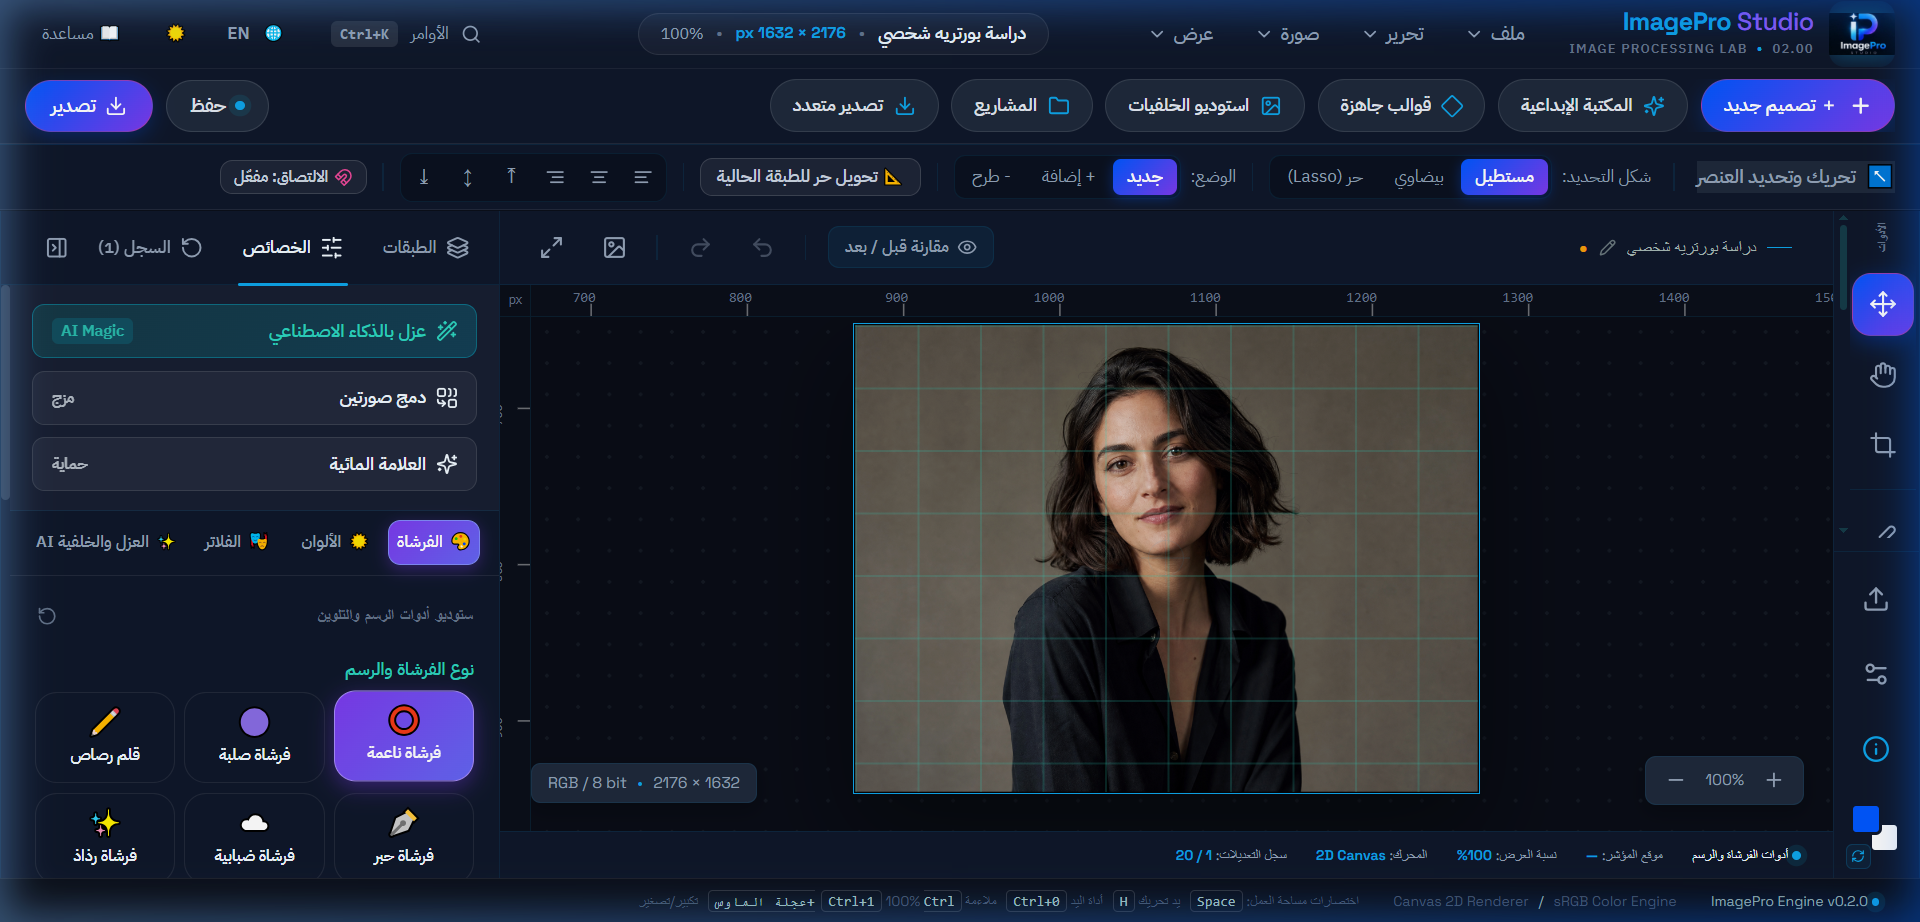
\includegraphics[width=0.85\textwidth]{11_drawing_brush_engine.png}
    \caption{محرك الفرشاة التنعيمية والرسم الرقمي وتخصيص الأشكال -- التحديث الأخير}
    \label{fig:drawing-engine}
\end{figure}

\begin{techbox}{شرح محرك الرسم والفرشاة التنعيمية (الشكل \ref{fig:drawing-engine})}
    لقطة حية من التحديث الأخير توضح تفاصيل محرك الفرشاة التنعيمية:
    \begin{itemize}
        \item \textbf{أنماط الفرشاة الأربعة:}
        \begin{enumerate}
            \item \textbf{فرشاة مستديرة ناعمة (Soft Round):} حواف غوسية متدرجة للتظليل والدمج.
            \item \textbf{فرشاة مستديرة صلبة (Hard Round):} حواف قاطعة 100\% للتحديد والرسم التقني.
            \item \textbf{ريشة الخط والحبر (Calligraphy/Ink):} زوايا متغيرة لمحاكاة أقلام الخط العربي.
            \item \textbf{مرذاذ الهواء (Airbrush/Spray):} توزيع احتمالي لنقاط اللون لمحاكاة الرش الفني.
        \end{enumerate}
        \item \textbf{منزلقات التحكم الفيزيائي:} منزلق الحجم (من 1 إلى 200 بكسل)، منزلق صلابة الحواف (Hardness \%)، منزلق العتامة والتدفق (Opacity \%)، ومنزلق التنعيم الذكي (Smoothing \%).
        \item \textbf{خوارزمية التنعيم بنقاط المنتصف التربيعية (Bezier Midpoint Smoothing):} تمنع الرعشة اليدوية بحساب نقاط وسطية ورسم منحنيات بيزيه ناعمة بين النقاط المتتالية للفأرة.
        \item \textbf{خوارزمية الملء الفيضاني (BFS Flood Fill):} طابور استكشاف رباعي الاتجاه في الذاكرة لمقارنة المسافة اللونية الإقليدية مع نسبة التسامح.
        \item \textbf{محدد الألوان السريع:} عينات الألوان الأكثر استخداماً ومنتقي الألوان المتدرج.
    \end{itemize}
\end{techbox}

\section{نافذة إعادة تحجيم أبعاد الصورة (Image Resize Dialog)}

\begin{figure}[htbp]
    \centering
    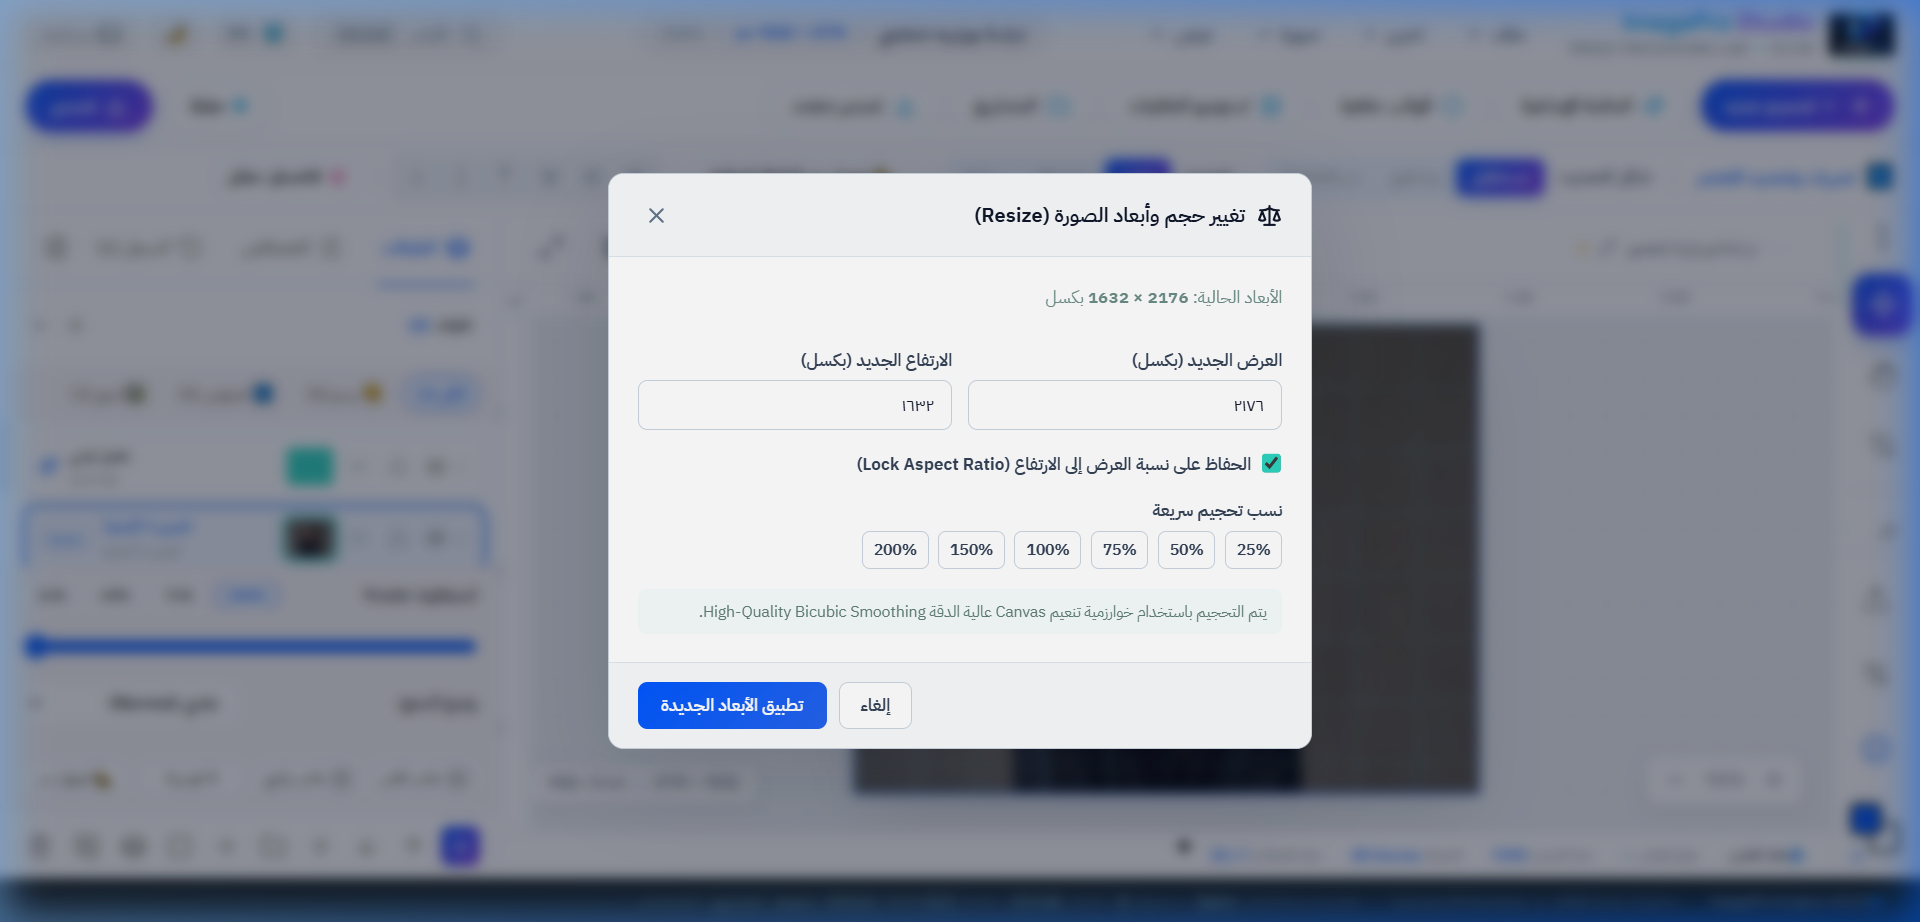
\includegraphics[width=0.85\textwidth]{19_resize_dialog.png}
    \caption{نافذة «تغيير حجم وأبعاد الصورة» مع قفل نسبة التناسب التلقائي}
    \label{fig:resize-dialog}
\end{figure}

\begin{techbox}{تفصيل نافذة التحجيم ومحرك الاستيفاء (الشكل \ref{fig:resize-dialog})}
    واجهة هندسية دقيقة لإعادة تشكيل أبعاد العمل الفني:
    \begin{itemize}
        \item \textbf{حقول الأبعاد بالبكسل:} إدخال العرض المستهدف (Width) والارتفاع المستهدف (Height).
        \item \textbf{أيقونة قفل التناسب الهندسي (Constrain Aspect Ratio):} الحفاظ التلقائي على نسبة الأبعاد الأصلية لمنع تشويه الصور.
        \item \textbf{أزرار النسب المئوية السريعة:} أزرار التصغير (50\%، 75\%) ومضاعفة الحجم (150\%، 200\%) بنقرة واحدة.
        \item \textbf{محرك الاستيفاء ثنائي الخطية (Bilinear Resampling Engine):} يقوم بحساب المتوسط الموزون للبكسلات الأربعة المجاورة لمنع التسنن وضمان النعومة البصرية.
    \end{itemize}
\end{techbox}

% ═════════════════════════════════════════════════════════════════════
% الفصل السابع: استوديو الذكاء الاصطناعي وشبكة IS-Net العصبية
% ═════════════════════════════════════════════════════════════════════
\chapter{استوديو الذكاء الاصطناعي وشبكة IS-Net العصبية}

\section{نموذج IS-Net (Dichotomous Image Segmentation)}
يوظف النظام شبكة عصبية عميقة تلافيفية متخصصة في التجزئة البصرية الثنائية فائقة الدقة لتفريغ الأجسام وعزل العناصر عن خلفياتها بدقة تشمل أدق التفاصيل كخصلات الشعر والأقمشة الشفافة.

\begin{figure}[htbp]
    \centering
    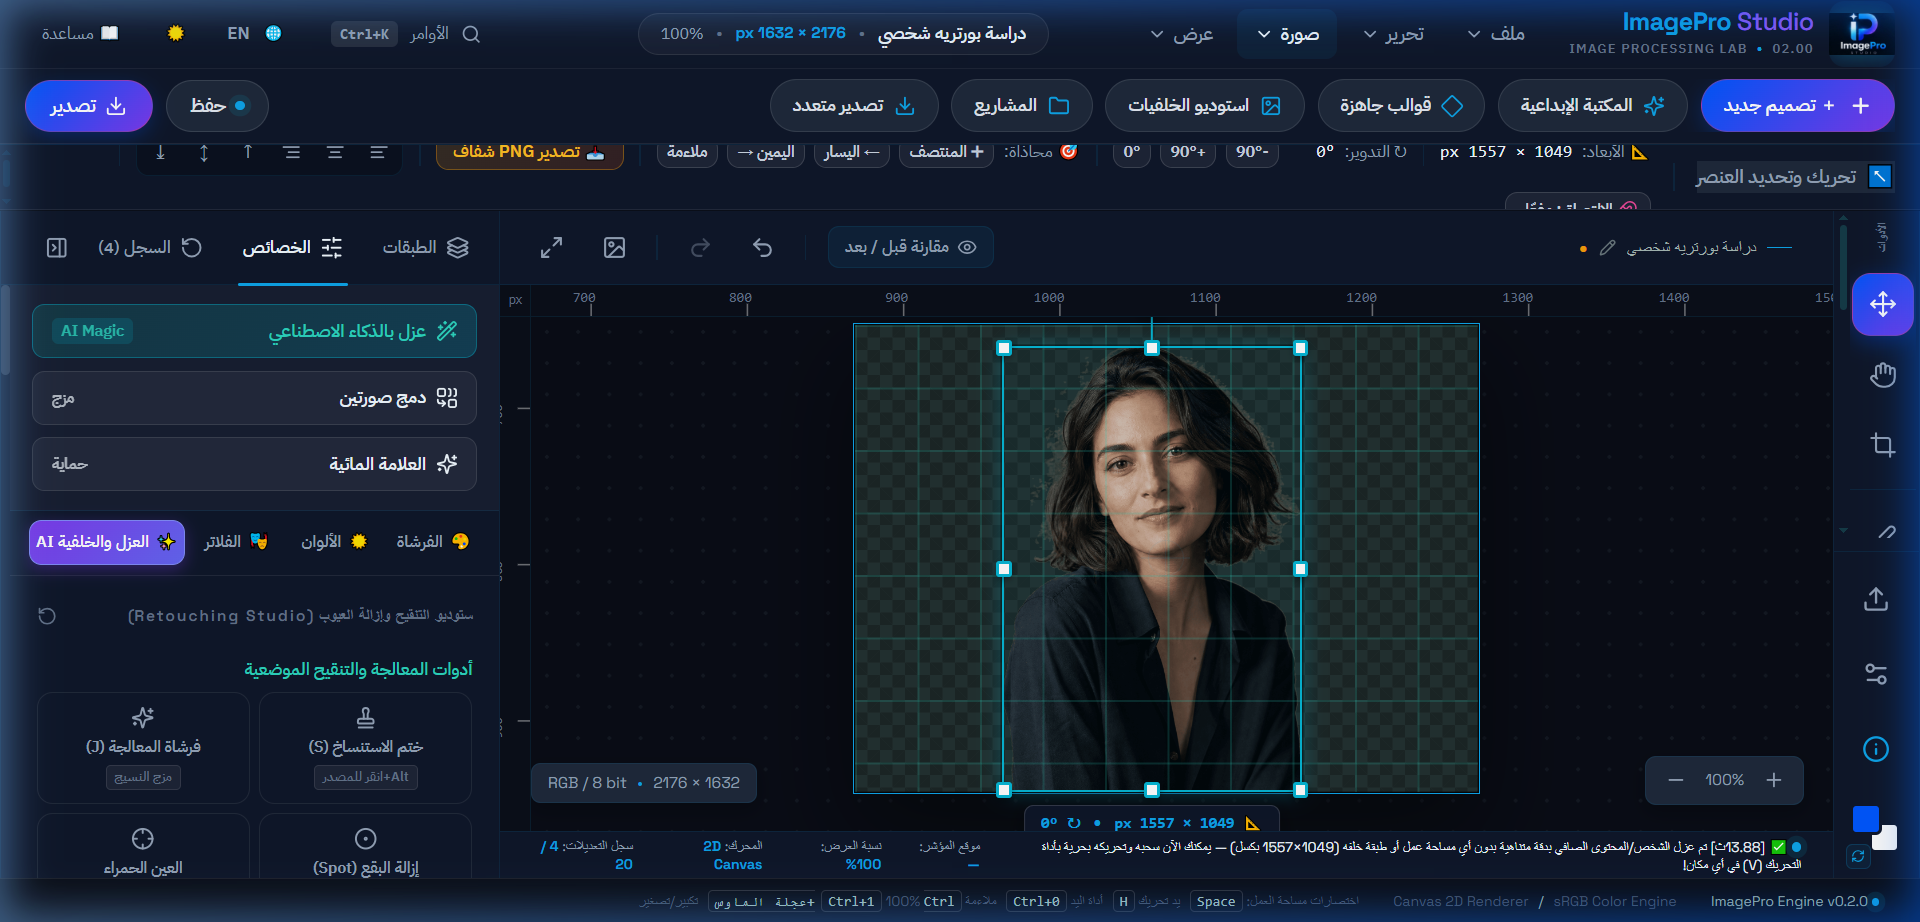
\includegraphics[width=0.85\textwidth]{12_ai_background_removal.png}
    \caption{استوديو الذكاء الاصطناعي وإعدادات العزل والتفريغ -- التحديث الأخير}
    \label{fig:ai-tab}
\end{figure}

\begin{techbox}{تفصيل استوديو الذكاء الاصطناعي وأنماط العزل (الشكل \ref{fig:ai-tab})}
    لقطة حية من التحديث الأخير تبرز واجهة استوديو الذكاء الاصطناعي (AI Magic Studio):
    \begin{itemize}
        \item \textbf{شارة الذكاء الاصطناعي الفائقة:} مؤشر تفعيل نموذج الشبكة العصبية العميقة IS-Net عبر WebAssembly و ONNX Runtime.
        \item \textbf{بطاقات أوضاع العزل الذكي الأربعة:}
        \begin{enumerate}
            \item \textbf{عزل مفرغ نقي (Transparent PNG Cutout):} استخراج العنصر كطبقة مفرغة نقية مع قناع ألفا كامل (Alpha Matte).
            \item \textbf{تمويه البورتريه السينمائي (Portrait Bokeh):} تمويه الخلفية بانسيابية تحاكي عدسات $f/1.4$ مع بقاء الجسم حاداً بنسبة 100\%، مع منزلق نصف قطر التمويه (Bokeh Radius).
            \item \textbf{استبدال بلون استوديو نقي (Solid Color Background):} أبيض نقي للمتاجر، أسود فخم، أو كروما خضراء للتأثيرات.
            \item \textbf{استبدال بصورة خلفية مخصصة (Custom Backdrop):} رفع أي صورة مشهدية لتصبح خلفية جديدة للعنصر المعزول بنقرة واحدة.
        \end{enumerate}
        \item \textbf{خيارات التحسين المتقدمة:} خيار إزالة الهالات الملونة والشوائب (Defringe / Anti-Color Spill) لضمان اندماج العنصر في الخلفية الجديدة بصورة طبيعية تماماً.
        \item \textbf{زر الإجراء «عزل الخلفية الآن»:} تشغيل المعالجة العصبية اللحظية وإدراج النتيجة كطبقة مستقلة.
    \end{itemize}
\end{techbox}

% ═════════════════════════════════════════════════════════════════════
% الفصل الثامن: العلامة المائية ومحرك التصدير متعدد المقاسات
% ═════════════════════════════════════════════════════════════════════
\chapter{العلامة المائية ومحرك التصدير متعدد المقاسات}

\section{استوديو العلامة المائية (Watermark Studio)}

\begin{figure}[htbp]
    \centering
    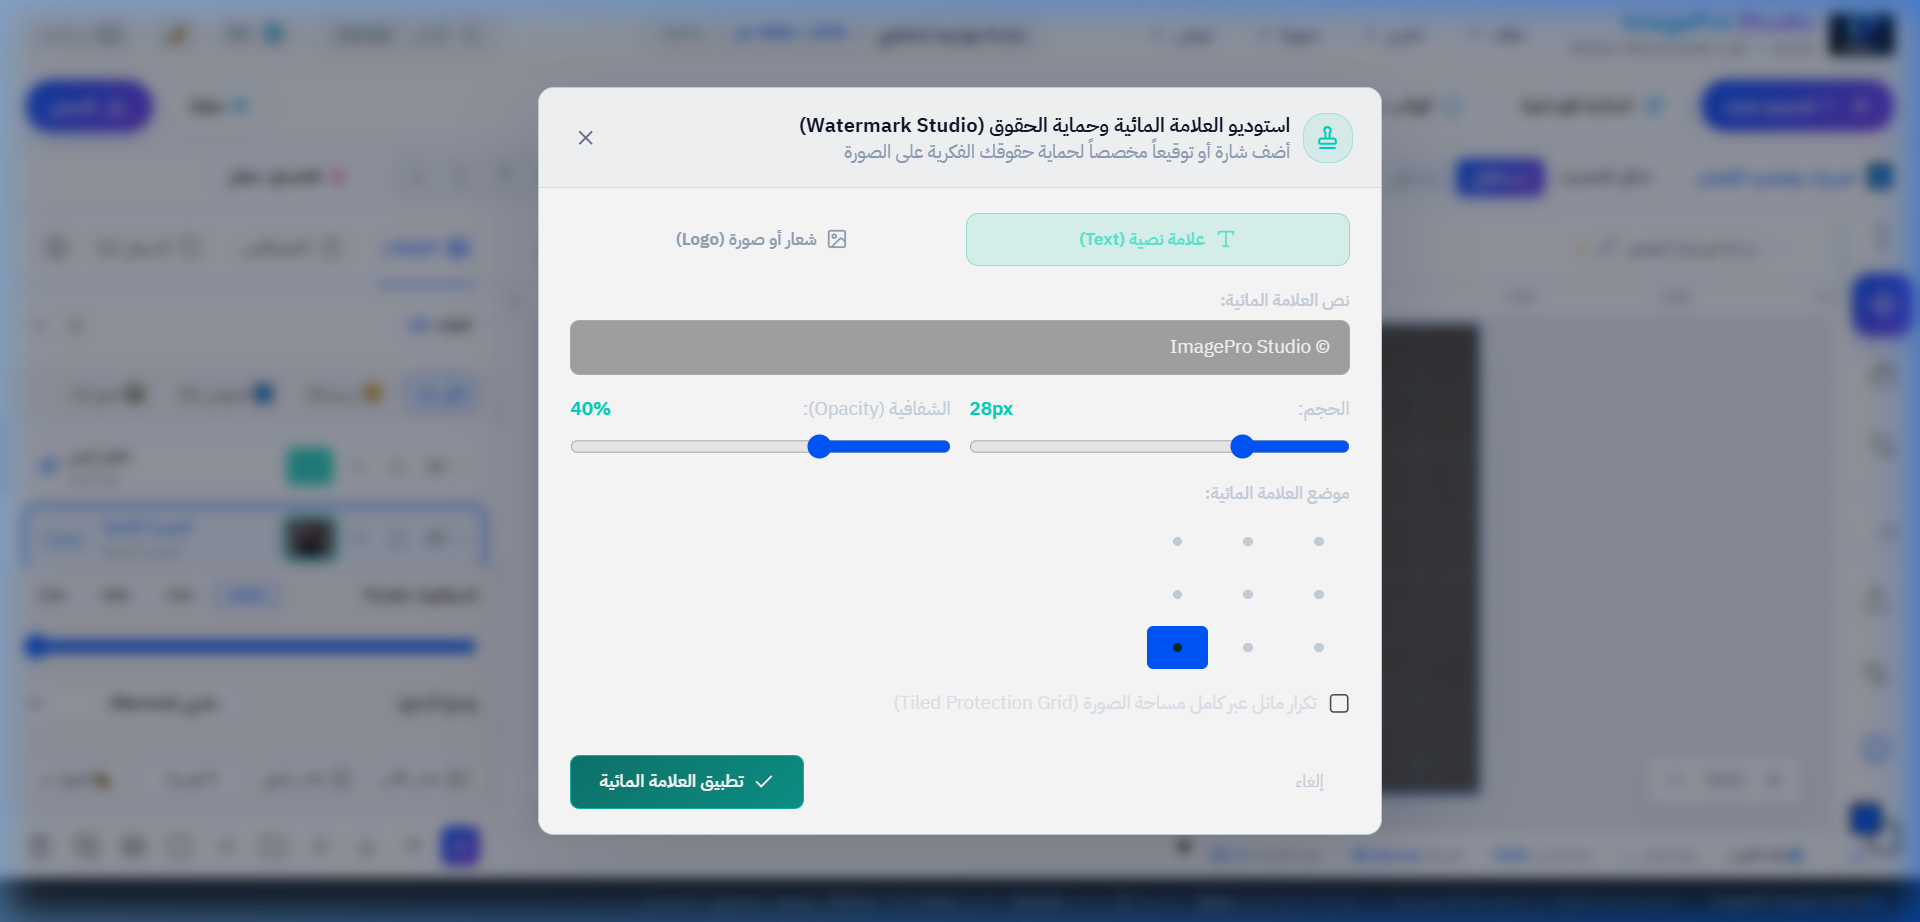
\includegraphics[width=0.88\textwidth]{17_watermark_studio.png}
    \caption{استوديو العلامة المائية لحماية الحقوق الفكرية بالنصوص والشعارات}
    \label{fig:watermark-studio}
\end{figure}

\begin{techbox}{أدوات وخصائص استوديو العلامة المائية (الشكل \ref{fig:watermark-studio})}
    يوفر للمصورين والشركات حماية متقدمة لصورهم وأعمالهم الفنية:
    \begin{itemize}
        \item \textbf{تبويب العلامة النصية:} حقل إدخال النص، اختيار نوع الخط العربي واللاتيني، تحديد الحجم، اللون، ونسبة العتامة.
        \item \textbf{تبويب الشعار الرسومي:} رفع ملف الشعار المفرغ بصيغة PNG مع منزلقات التحجيم والتدوير.
        \item \textbf{نمط التكرار الشبكي المائل (Diagonal Tile Pattern):} تكرار العلامة مصفوفياً بزاوية $45^\circ$ لتغطية كامل مساحة العمل لمنع القص والسرقة الفكرية.
        \item \textbf{أزرار التموضع السريع:} وضع العلامة في الزوايا الأربع أو في المركز بنقرة واحدة.
    \end{itemize}
\end{techbox}

\section{محرك التصدير متعدد المقاسات (Multi-Size Export Hub)}

\begin{figure}[htbp]
    \centering
    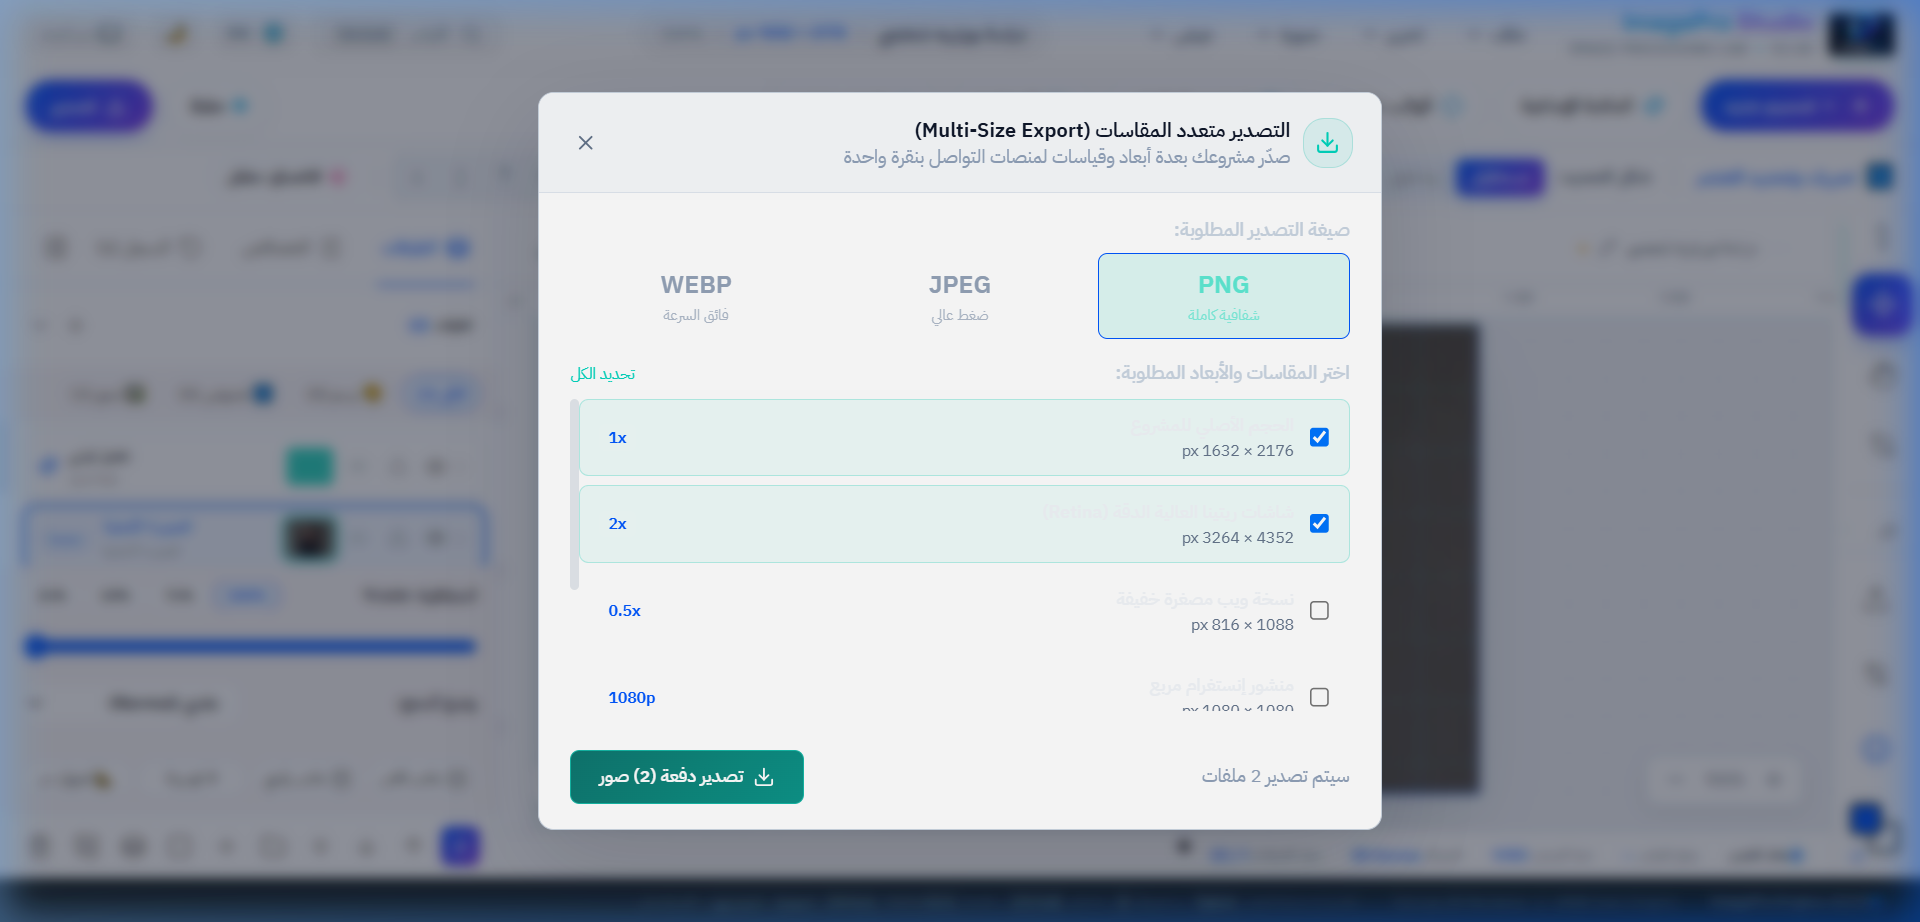
\includegraphics[width=0.88\textwidth]{18_multisize_export.png}
    \caption{محرك التصدير متعدد المقاسات لإنتاج حزم السوشيال ميديا وحفظها في ملف مضغوط ZIP}
    \label{fig:multisize-export}
\end{figure}

\begin{techbox}{شرح وميزات محرك التصدير المتعدد (الشكل \ref{fig:multisize-export})}
    محرك إنتاجي يقوم بتوليد كافة مقاسات منصات التواصل دفعة واحدة:
    \begin{itemize}
        \item \textbf{قائمة المنصات المدعومة:} Instagram Post, Instagram Story, Facebook Post, Twitter Banner, YouTube Thumbnail, LinkedIn Banner.
        \item \textbf{تنسيقات الملفات المخرجة:} صيغة PNG الشفافة، صيغة JPEG مع منزلق نسبة الجودة والضغط، وصيغة WebP الحديثة للويب.
        \item \textbf{الحزم في ملف مضغوط واحد (Instant ZIP Archive):} توليد الصور في الذاكرة وضغطها في ملف \texttt{.zip} مجهز للتحميل المباشر.
    \end{itemize}
\end{techbox}

% ═════════════════════════════════════════════════════════════════════
% الفصل التاسع: مصفوفة الاختبارات الآلية وضمان الجودة (70 اختباراً)
% ═════════════════════════════════════════════════════════════════════
\chapter{بيئة الاختبارات وضمان الجودة البرمجية}

يخضع النظام لنظام اختبارات تكاملي ووحدي آلي مبني على منصة \textbf{Vitest 2.1}، حيث تجتاز الشيفرة البرمجية \textbf{70 اختبار وحدة عبر 16 ملف اختبار بنسبة نجاح 100\%}.

\begin{table}[htbp]
    \centering
    \caption{سجل نتائج الاختبارات الآلية الشاملة (100\% Success Rate)}
    \label{tab:tests-matrix}
    \begin{tabularx}{\textwidth}{l X c c}
        \toprule
        \textbf{ملف الاختبار البرمجي} & \textbf{نطاق الفحص والتحقق الهندسي} & \textbf{عدد الاختبارات} & \textbf{الحالة} \\
        \midrule
        \texttt{phase5-layers.test.ts} & معمارية الطبقات، المزج، والأقنعة غير التدميرية & 14 & \textcolor{StudioGreen}{\textbf{✅ ناجح}} \\
        \texttt{retouch-engine.test.ts} & أدوات التنقيح (الختم، المعالجة، تنعيم البشرة) & 7 & \textcolor{StudioGreen}{\textbf{✅ ناجح}} \\
        \texttt{selection.test.ts} & محرك التحديد الهندسي والعمليات المنطقية & 7 & \textcolor{StudioGreen}{\textbf{✅ ناجح}} \\
        \texttt{subject-extractor.test.ts} & نموذج الذكاء الاصطناعي، العزل، والبوكيه & 6 & \textcolor{StudioGreen}{\textbf{✅ ناجح}} \\
        \texttt{filters-engine.test.ts} & الفلاتر الـ 21 والالتفاف المكاني ثنائي الأبعاد & 5 & \textcolor{StudioGreen}{\textbf{✅ ناجح}} \\
        \texttt{smart-drop-hub.test.ts} & مركز السحب والإفلات وتوجيه الأصول & 5 & \textcolor{StudioGreen}{\textbf{✅ ناجح}} \\
        \texttt{guides-snap-engine.test.ts} & المساطر التفاعلية والمغنطة والمحاذاة الذكية & 4 & \textcolor{StudioGreen}{\textbf{✅ ناجح}} \\
        \texttt{drawing-engine.test.ts} & الفرشاة التنعيمية، أقواس بيزيه، والملء الفيضاني & 3 & \textcolor{StudioGreen}{\textbf{✅ ناجح}} \\
        \texttt{color-adjustments.test.ts} & التعديلات الضوئية، فضاء HSL، والهستوجرام & 3 & \textcolor{StudioGreen}{\textbf{✅ ناجح}} \\
        \texttt{project-persistence.test.ts} & تشفير وحزم ملفات المشاريع (\texttt{.imagepro}) & 3 & \textcolor{StudioGreen}{\textbf{✅ ناجح}} \\
        \texttt{autosave-manager.test.ts} & الحفظ التلقائي المحلي وسجل استعادة النسخ & 3 & \textcolor{StudioGreen}{\textbf{✅ ناجح}} \\
        \texttt{creative-backgrounds.test.ts} & كتالوج الخلفيات الإبداعية الـ 17 فئة & 2 & \textcolor{StudioGreen}{\textbf{✅ ناجح}} \\
        \texttt{product-backgrounds.test.ts} & استوديو خلفيات المنتجات وتصيير الكانفاس & 2 & \textcolor{StudioGreen}{\textbf{✅ ناجح}} \\
        \texttt{editable-templates.test.ts} & القوالب متعددة الطبقات وهياكل المكونات & 2 & \textcolor{StudioGreen}{\textbf{✅ ناجح}} \\
        \texttt{templates.test.ts} & المقاسات القياسية ومنصات النشر الرقمي & 2 & \textcolor{StudioGreen}{\textbf{✅ ناجح}} \\
        \texttt{tool-contract.test.ts} & تكامل عقود الأدوات والتزامن مع الواجهة & 2 & \textcolor{StudioGreen}{\textbf{✅ ناجح}} \\
        \midrule
        \textbf{المجموع الكلي} & \textbf{تغطية برمجية شاملة لكافة محركات النظام} & \textbf{70} & \textcolor{StudioGreen}{\textbf{✅ 70/70 بنجاح تام}} \\
        \bottomrule
    \end{tabularx}
\end{table}

علاوة على ذلك، يتم إجراء فحص الأنواع الصارم للغة TypeScript عبر الأمر \texttt{tsc --noEmit} محققاً \textbf{0 أخطاء برمجية}.

% ═════════════════════════════════════════════════════════════════════
% الفصل العاشر: الخاتمة والتوصيات المستقبلية
% ═════════════════════════════════════════════════════════════════════
\chapter{الخاتمة والتوصيات المستقبلية}

\section{الخاتمة الهندسية}
يقدم مشروع \textbf{ImagePro Studio} برهاناً عملياً وهندسياً متقدماً على إمكانية تطوير تطبيقات معالجة صور وتصميم رسومي فائقة القوة عبر تقنيات الويب الحديثة، مع دعم كامل للوضعين النهاري والليلي وتجربة مستخدم لا تضاهى.

\section{التوصيات وآفاق التطوير المستقبلي}
\begin{enumerate}
    \item \textbf{تسريع الحوسبة عبر WebGPU:} نقل نوى الالتفاف الرياضي ومعالجة الفلاتر من معالج الكانفاس إلى كروت الشاشة عبر شفرات Compute Shaders.
    \item \textbf{التعاون اللحظي متعدد المستخدمين (Real-Time Collaboration):} دمج خوارزميات CRDTs ومقبس WebSockets لتمكين عدة مصممين من العمل على نفس المشروع بشكل متزامن.
    \item \textbf{توسيع استوديو الذكاء الاصطناعي التوليدي:} دمج نماذج Inpainting لنشر الأنسجة الذكية والترميم التلقائي للصور التالفة.
\end{enumerate}

\vspace{1.5cm}
\begin{center}
    \begin{tcolorbox}[colback=StudioLight,colframe=StudioPrimary,arc=3mm,width=0.9\textwidth,center]
        \centering \bfseries \large
        تم بحمد الله إعداد وتوثيق هذا التقرير التقني الشامل لمشروع التخرج\\[0.3cm]
        \textcolor{StudioPrimary}{فريق الإعداد والتطوير الهيكلي:}\\[0.2cm]
        سليمان العربي \quad • \quad يعقوب المهاجري \quad • \quad مالك عادل
    \end{tcolorbox}
\end{center}

\end{document}
